
\chapter{Charge Ratio of Atmospheric Muons at IICHEP-Madurai}


The study of atmospheric muon charge ratio
$\left(R_{\mu}=N_{\mu^{+}}/N_{\mu^{-}}\right)$
is important to the measurement of the neutrino flux precisely,
alongside the relevant information in the composition of the primary
cosmic rays and the different mechanisms of matter particle
interactions.

The shower of secondary particles consists mainly of
\mbox{pions $\left(\pi^{\pm}, \pi^0\right)$} and
\mbox{kaons $\left(K^{\pm}, K^0_S, K^0_L\right)$} which are produced due
the interactions of primary cosmic rays consisting of mainly proton
and a small fraction of higher $Z$ atoms \cite{cosmic1,pdgspectra1}
with atmospheric nuclei at the upper atmosphere (mostly at 15-20\,km
altitude).
The neutral pions mainly decay via electro-magnetic interactions,
$\pi^0 \rightarrow \gamma+\gamma$ whereas the charged pions decay to
muons and neutrinos via weak-interactions,
$\pi^+ \rightarrow \mu^+ + \nu_{\mu}$ and
$\pi^- \rightarrow \mu^- + \bar{\nu}_{\mu}$. The kaons also decay to
muons, neutrinos and to pions in different branching fractions.
Most of the pions and kaons decay in flight and do not reach the
earth's surface.
A small fraction of resultant muons decay into electrons and neutrinos,
$\mu^+ \rightarrow e^+ + \nu_{e} + \bar{\nu}_{\mu}$ and
$\mu^- \rightarrow e^- + \bar{\nu}_{e} + \nu_{\mu}$.
The $\gamma$, $e^{\pm}$ do not reach the detector directly as they
interact with atmospheric nuclei as well as the roof of the laboratory
and generate electromagnetic showers, which can be easily distinguished
from the muon trajectory in the RPC stack.

Hence, the cosmic ray muons are the most abundant charged particles
available at the surface of the earth. The relativistic muons lose
about 2\,GeV in ionisation before reaching the sea level.
As the primary cosmic rays are dominated by the proton, air molecule
  contains proton and neutron, the production of the positively
  charged kaons/pions/muons are more favoured.
Hence the muon charge ratio reflects the excess of $\pi^{+}$ over
$\pi^{-}$ and $K^{+}$ over $K^{-}$ during the formation of the
cosmic ray shower in the forward region. In the TeV range however,
the associated production of $K^{+}$
($p+air \rightarrow K^{+} + \Lambda + ...$), which has no analog for $K^{-}$,
largely favours $K^{+}$ production over $K^{-}$, making the
$K^{+}$/$K^{-}$ ratio greater than $\pi^{+}$/$\pi^{-}$ ratio
\cite{adamson2007}.
%\[p+\text{air} \rightarrow K^{+} + \Lambda + \text{...}\]

Thus the charge ratio increases with the increasing kaon contribution
with the increasing energy of the primary cosmic rays.
The measurement of the charge ratio in TeV range thus, allow to limit
the production of kaons inaccessible to the collider experiments
at present, which is essential for better prediction of neutrino
flux and $\nu_{\mu}/\bar{\nu}_{\mu}$ ratio.

One of the main aspects of ICAL detector is to distinguish between
the $\mu^{+}$ and $\mu^{-}$ passing through the magnetised iron
medium, which is required in determining the mass-hierarchy of
the neutrinos with low statistics cosmic neutrino events.
So before deploying the main ICAL, a few prototypes
of the detector are planned to be build in order to test various
aspects.
As a part of the ICAL R\&D program, a magnetised detector (mini-ICAL)
with 10 layers of RPCs has been built and operational at IICHEP,
Madurai situated near the INO site. Being a scale-down model of the
ICAL detector, the mini-ICAL is being studied as the prototype of
the magnetised ICAL. This prototype is mainly built to study the
performance of electronics equipment in the presence of the magnetic
field and to test the event reconstruction algorithms.
The cosmic ray data collected by the
detector setup is also used to calculate the charge ratio $(R)$
of the number of $\mu^{+}$ to $\mu^{-}$ arriving at the Earth's surface.
The testing of the INO-ICAL muon reconstruction algorithms is also
another motivation behind this study.
By comparing the result from cosmic ray data with extreme
air shower (EAS) simulation, this study also signifies the ability of
the magnet in identifying the charge of the particle.

\section{Detector Setup of mini-ICAL}
The present setup, named mini-ICAL, is a magnetised iron calorimeter
weighing at 85\,Tonn. The mini-ICAL detector consists of 11 layers
of iron of size 4\,m\,$\times$\,4\,m\,$\times$\,5.6\,cm with the
inter-layer gap of 4.5\,cm. This makes the dimensions of this
prototype detector are 4\,m\,$\times$\,4\,m\,$\times$\,1.06\,m.
The detector setup is shown in the Figure~\ref{fig:miniICAL_iron}
%% where the $X$-axis of the detector is making an angle of $10^\circ$
%% with the geographic north
.
\begin{figure}[h]
  \centering
  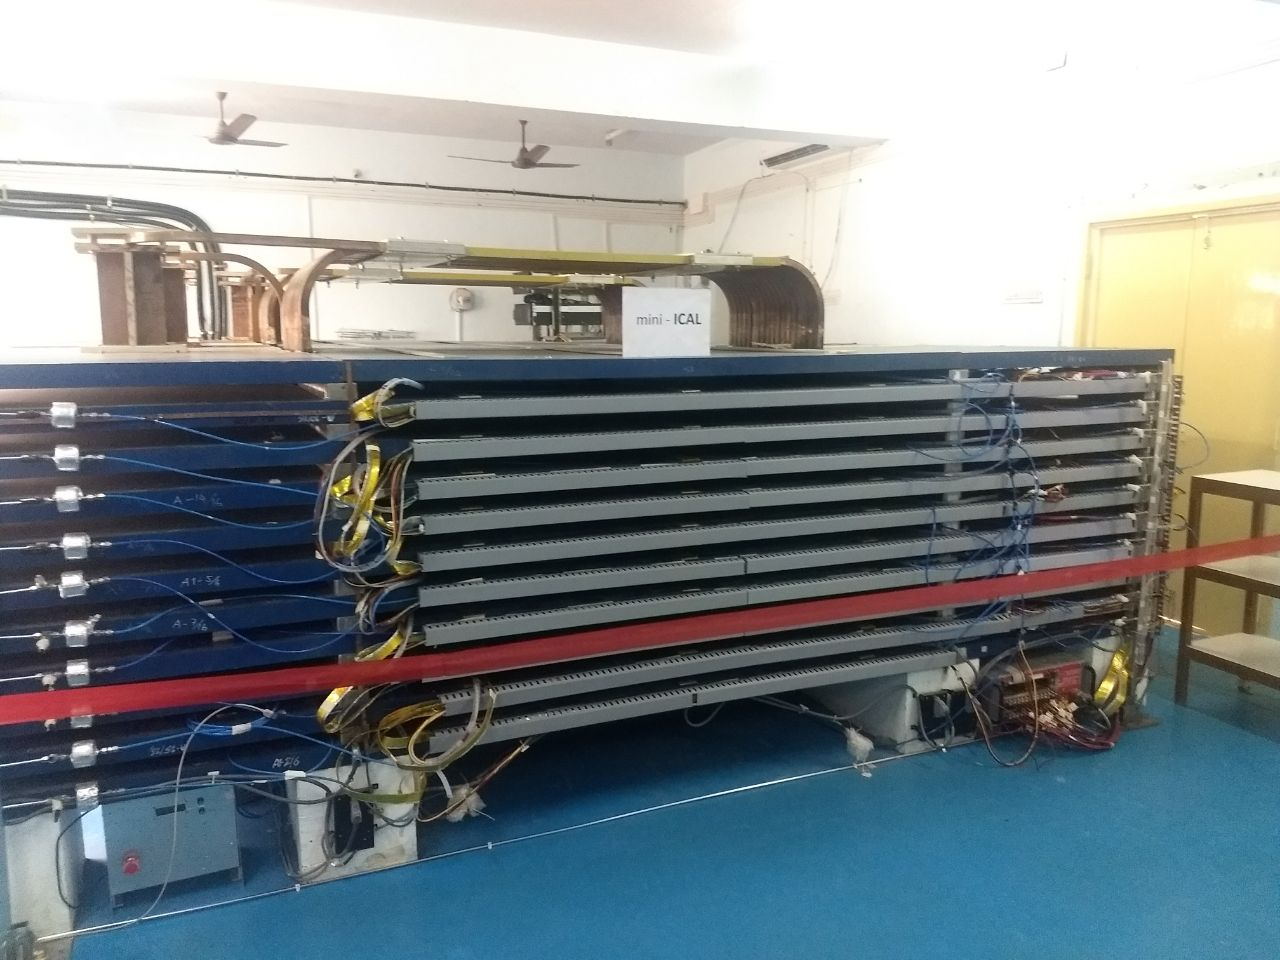
\includegraphics[width=0.49\linewidth]{micalphoto.png}
  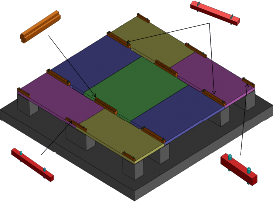
\includegraphics[width=0.49\linewidth]{miniICAL_iron_block.pdf}
  \caption{(Left) The mini-ICAL Detector Setup (right) and the
    different sections of one layer of iron and the stainless-steel
    spacers.}
  \label{fig:miniICAL_iron}
\end{figure}
The iron layers in the mini-ICAL magnet is made of soft iron with
the additional chemical composition of C\,(0.015\%), Mn\,(0.37\%),
P\,(0.012\%), S\,(0.008\%), Si\,(0.188\%), Al\,(0.001\%), N\,(50\,ppm). %GMA fraction is more in N than Al ? SNM-> I took the values from Apoorva's thesi.
This soft iron has low carbon content which makes it strong enough
mechanically to support its own weight, but also allows it to have high
permeability with knee point at around $\sim$1.5\,T.
Each of the layers of iron consists of several different tiles shown
in the Figure~\ref{fig:miniICAL_iron}.
The gap between the layers are maintained with the help of the spacers
made of non-magnetic stainless steel (SS-304) are also shown in the
Figure~\ref{fig:miniICAL_iron}.

There are four slots with dimensions of 80\,cm\,$\times$\,8\,cm to
accommodate two sets of current conducting coils to generate magnetic
field inside the iron in a similar fashion to the proposed
ICAL detector. The coils are made of OFE-grade copper with
oxygen content less than 10\,ppm. There are 18 turns of coils in each
set of coils. Each of the turns are kept at a distance of 40\,mm.
The coils are hollow inside with the cross section of
30\,mm\,$\times$\,30\,mm\,$\times$\,$\phi$17\,mm.
The two sets of coils are electrically connected in series,
and a low voltage power supply is used to supply 900\,Amp
of trough via the coils. A uniform magnetic field of $\sim$1.5\,T
is obtained in the central region of the detector.
%%  The magnetic field
%% in the mini-ICAL is along the ($-$)Y-direction in the central region.
The strength of the magnetic field in the iron layer along the X- and Y-
axis are shown in the Figure~\ref{fig:magfieldmical}. It can be seen
that most of the field strength is present in the central region of the
detector along the (-)Y-direction.
\begin{figure}[h]
  \centering
  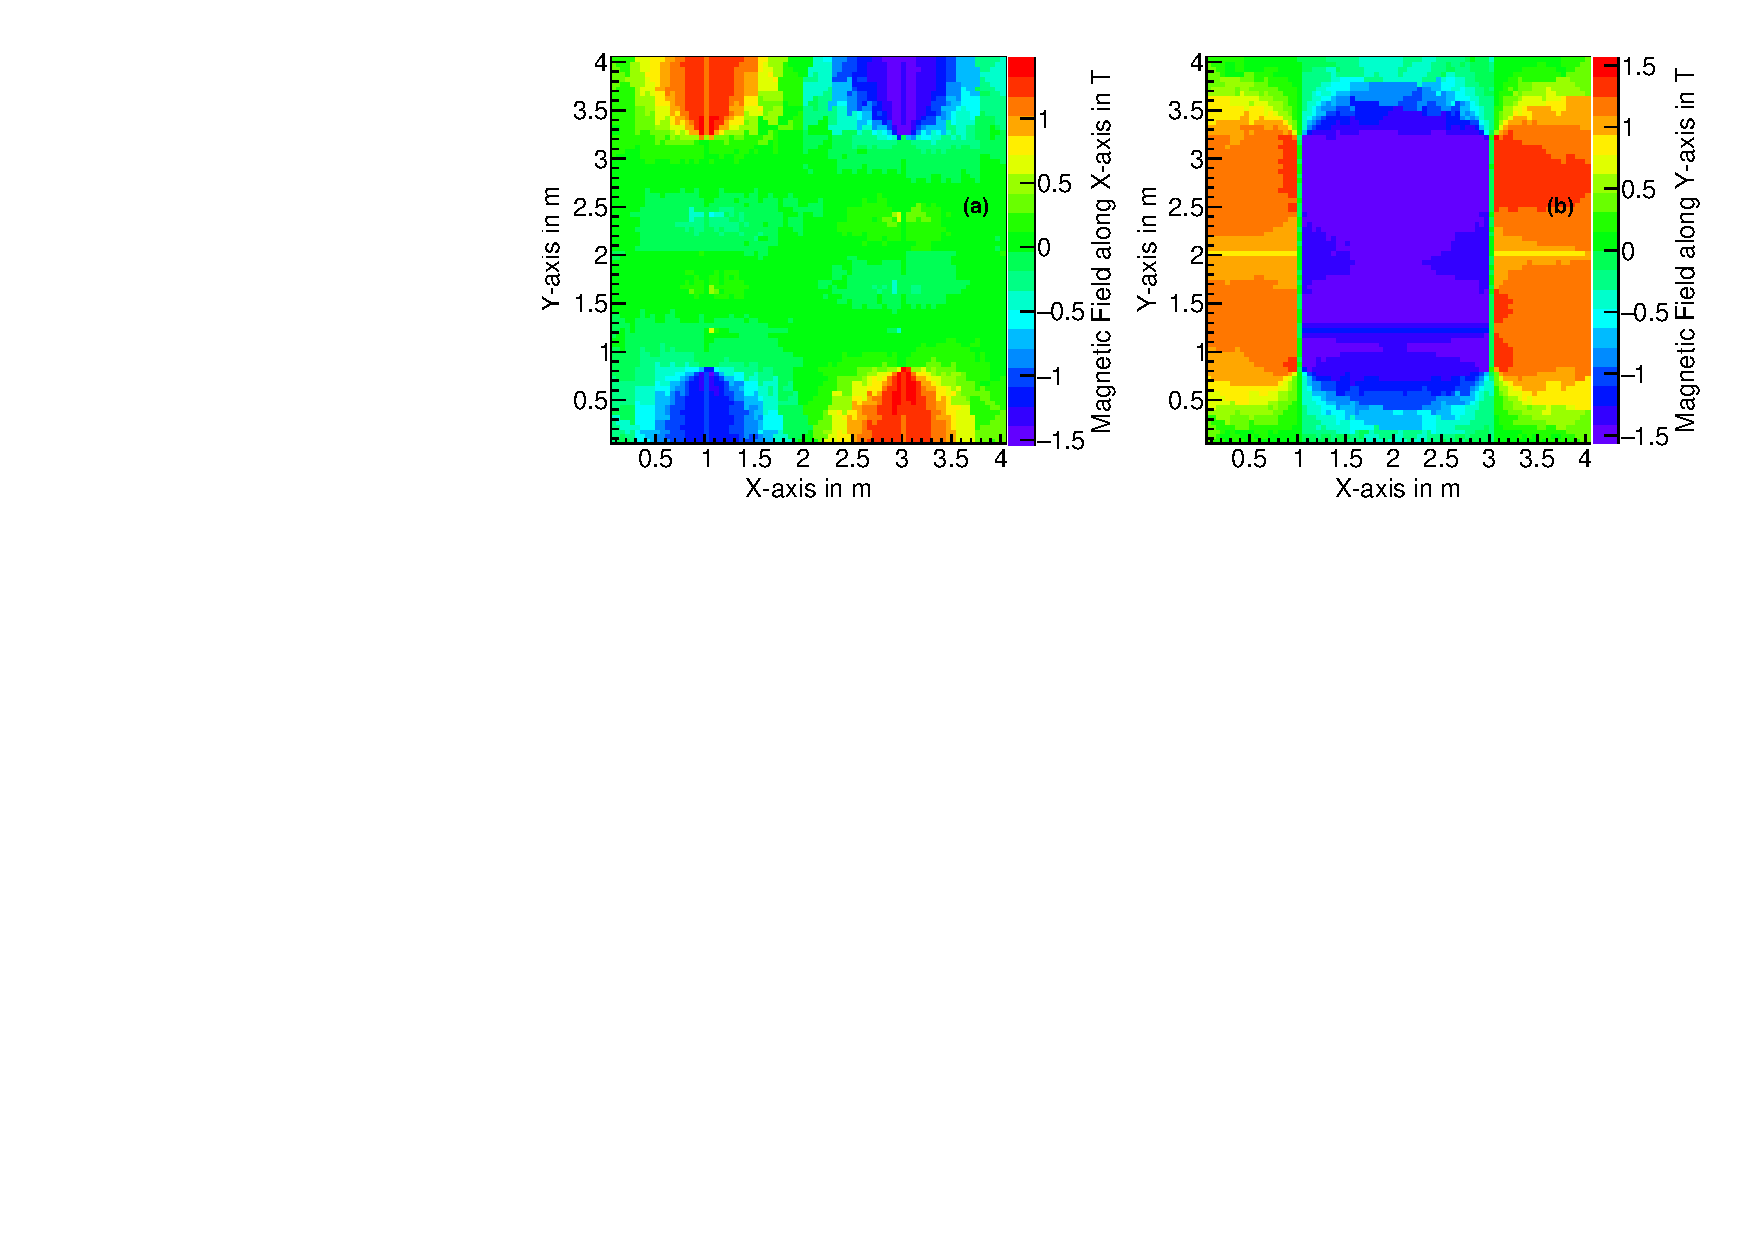
\includegraphics[width=0.9\linewidth]{mag_field_mICAL.pdf}
  \caption{The strength of magnetic field in the iron layer along (a) X-
    and (b) Y- axis.}
  \label{fig:magfieldmical}
\end{figure}

The heat generated by the current in the
coils are extracted by a closed-loop low conductivity water cooling
system (LCWCS) by flowing chilled water through the bore of the coils.

Ten RPCs of dimensions 174\,cm\,$\times$\,183.5\,cm are used as the
active detector. These RPCs are placed in the central region of
the detector in between iron layers.
An RPC gap is made of two glass electrodes of thickness 3\,mm with
a gap of 2\,mm between them. Uniform gap between these two electrodes
is maintained using an array of 2\,mm thick poly-carbonate buttons.
The glass gap is sealed on the outer edges to make it air-tight.
A mixture of gases with the compositions of R134a (95.2\%),
iso-C$_4$H$_{10}$ (4.2\%) and SF$_6$ (0.3\%) is flown in the RPCs
via strategically placed nozzles. This mixture of gasses serves as the
target medium of the detector.
Both the outer surfaces of the glass gap are coated with a thin layer
of graphite. The RPCs are operated by applying a differential supply of
$\pm$\,5\,kV to the graphite layers which creates a constant electric
field between the glass electrodes. The ionisation of the gas mixture
by passage of the charged particles eventually evolves into a
avalanche in the presence of the high electric field between the glass
electrodes. The avalanche in the RPCs induces signals in the two
orthogonal pickup panels placed on both sides of the glass gaps
labelled as X-side (bottom panel) and Y-side (top panel). The pickup panels
  are made of parallel
copper strips of width 28\,mm with 2\,mm gap between two consecutive
strips. There are 58 strips on the X-side and 61 strips on the %GMA 60 & 63 or 59 & 61 ? SNM-> 58 & 61
Y-side for each layer.

The DAQ system is similar to the setup discussed in the previous
chapter. In this case the cosmic muon data have been collected using
the 1-Fold signals from the top 4 layers as trigger.
An event data typically contains strip hit and timing information
of an event. The strip hit is basically one logic bit per strip
indicating the signal in that strip is above the threshold value
for that strip. The least count of each of the TDC is 0.1\,ns.
The timing data consist of 16 time signal for
each layer where each multi-hit TDC channel records time signals
coming from every alternate 8$^{th}$ strips on one side of the layer.
The time signal of each hit is recorded for both the leading-edge and
the trailing-edge of the induced signal pulse.

\section{Monte-Carlo Simulation}
The Monte-Carlo Simulation for this study has been executed in
two parts. The Extensive Air Shower (EAS) has been simulated
by the CORSIKA simulation package\cite{corsika763}. The information
of daughter particles generated by the EAS at the earth's surface
level has been extracted and used in the detector simulation.
The detector simulation has been executed with the help
of the GEANT4 toolkit\cite{geant4}. The schemes of the EAS and the
detector simulations are already elaborated in the
Chapter~\ref{chapter:multi}.

In this study, for simulating the behaviour of hadrons for higher
energy range, the SIBYLL has been adopted and
for the low energy range, the FLUKA model has been used
\cite{corsika763}. The primary cosmic ray shower has been simulated
using the CORSIKA(v7.6300) Package. The energy of the primary rays in
the CORSIKA is generated using the power-law spectrum, $E^{-2.7}$,
within the energy range of \mbox{$10$--$10^{6}$\,GeV}. The zenith and
azimuth angle of primary particles are generated uniformly within the
range of \mbox{$0$--$85^\circ$} and \mbox{$0$--$360^\circ$},
respectively. The magnetic rigidity cutoff has been implemented
according to the location of the detector.

An identical model of the detector including the building in which it
is housed, is prepared in the GEANT4 in order to perform the detector
simulation. The material in the simulation is chosen as per the
material present in the setup. The model of the setup in GEANT4 is
shown in the Figure~\ref{fig:miniICAL_view}.
\begin{figure}[h]
  \centering
  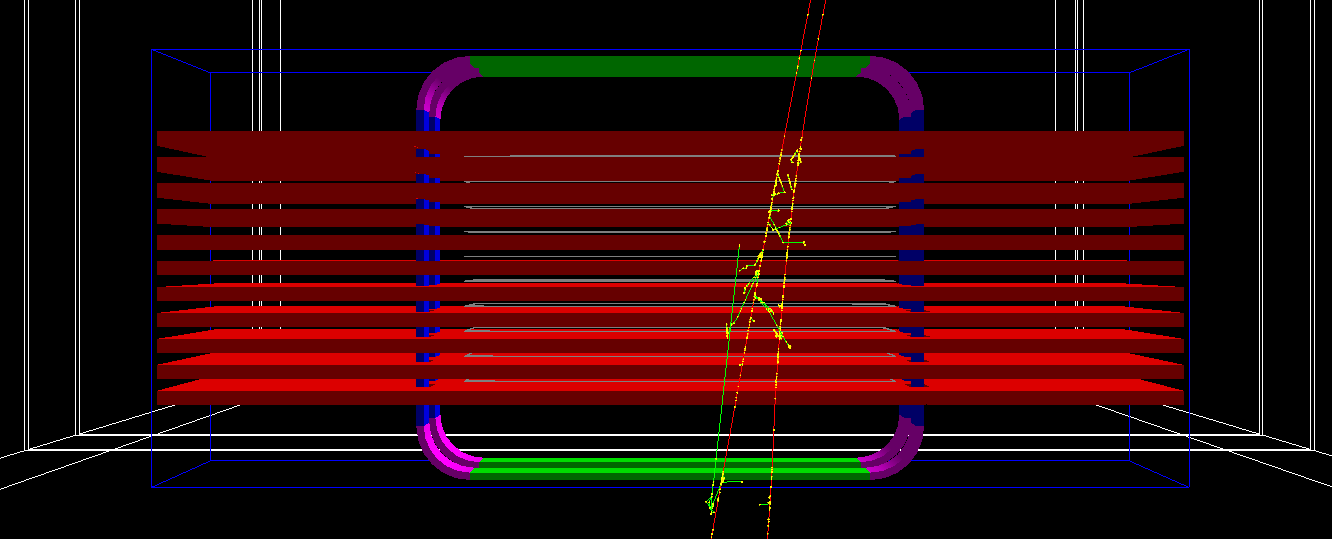
\includegraphics[width=0.99\linewidth]{mical_view.png}
  \caption{Model of the miniICAL magnet system in GEANT4.}
  \label{fig:miniICAL_view}
\end{figure}
In the detector simulation; the momentum value and the direction
of the muons are randomly generated from the CORSIKA spectra.
The detector's parameters (efficiency, noise, strip multiplicity and
resolution) are calculated using the cosmic ray data without magnetic
field in the detector.

Both the events from the observed cosmic ray data and the detector
simulation are reconstructed using the track fit algorithm which is
discussed in the next section.

\section{Event Reconstruction and Data Selection} \label{sec:momreco}
The recorded data is actually the projection of the track on the
\mbox{X--Z} and \mbox{Y--Z} sides. During the passage of a charged
particle through a RPC gap, the number of strips on which signal is
induced depends on the gain of the gas gap at the place of passing.
This sharing of the induced signal between the neighbouring strips is
one of the main reasons for the observed strip multiplicity shown in the
Figure~\ref{fig:layer2y}(c), whereas other reasons are streamer pulse
as well as correlated electronics noise.
In order to prepare the events for analysis, the consecutive strips
which have recorded signals are clubbed together to form a cluster.
The layers with no clusters either or both on X and Y sides are
neglected during the track reconstruction.

During the study, the position resolution for strip multiplicities of
1, 2 are $\sim$6\,mm. In this study, the clusters of hits with more
than 2 multiplicities are neglected as the position resolution for
higher multiplicities is found to be the worse. A layer which has
more than 15 strip hits and/or more than 10 clusters is tagged as
`noisy layer' and not considered in the track reconstruction. An
event which has more than 3 noisy layers is considered as a
`noisy event' and discarded.

A few such events are displayed in the Figure~\ref{fig:eventdisplay}.
\begin{figure}[h]
  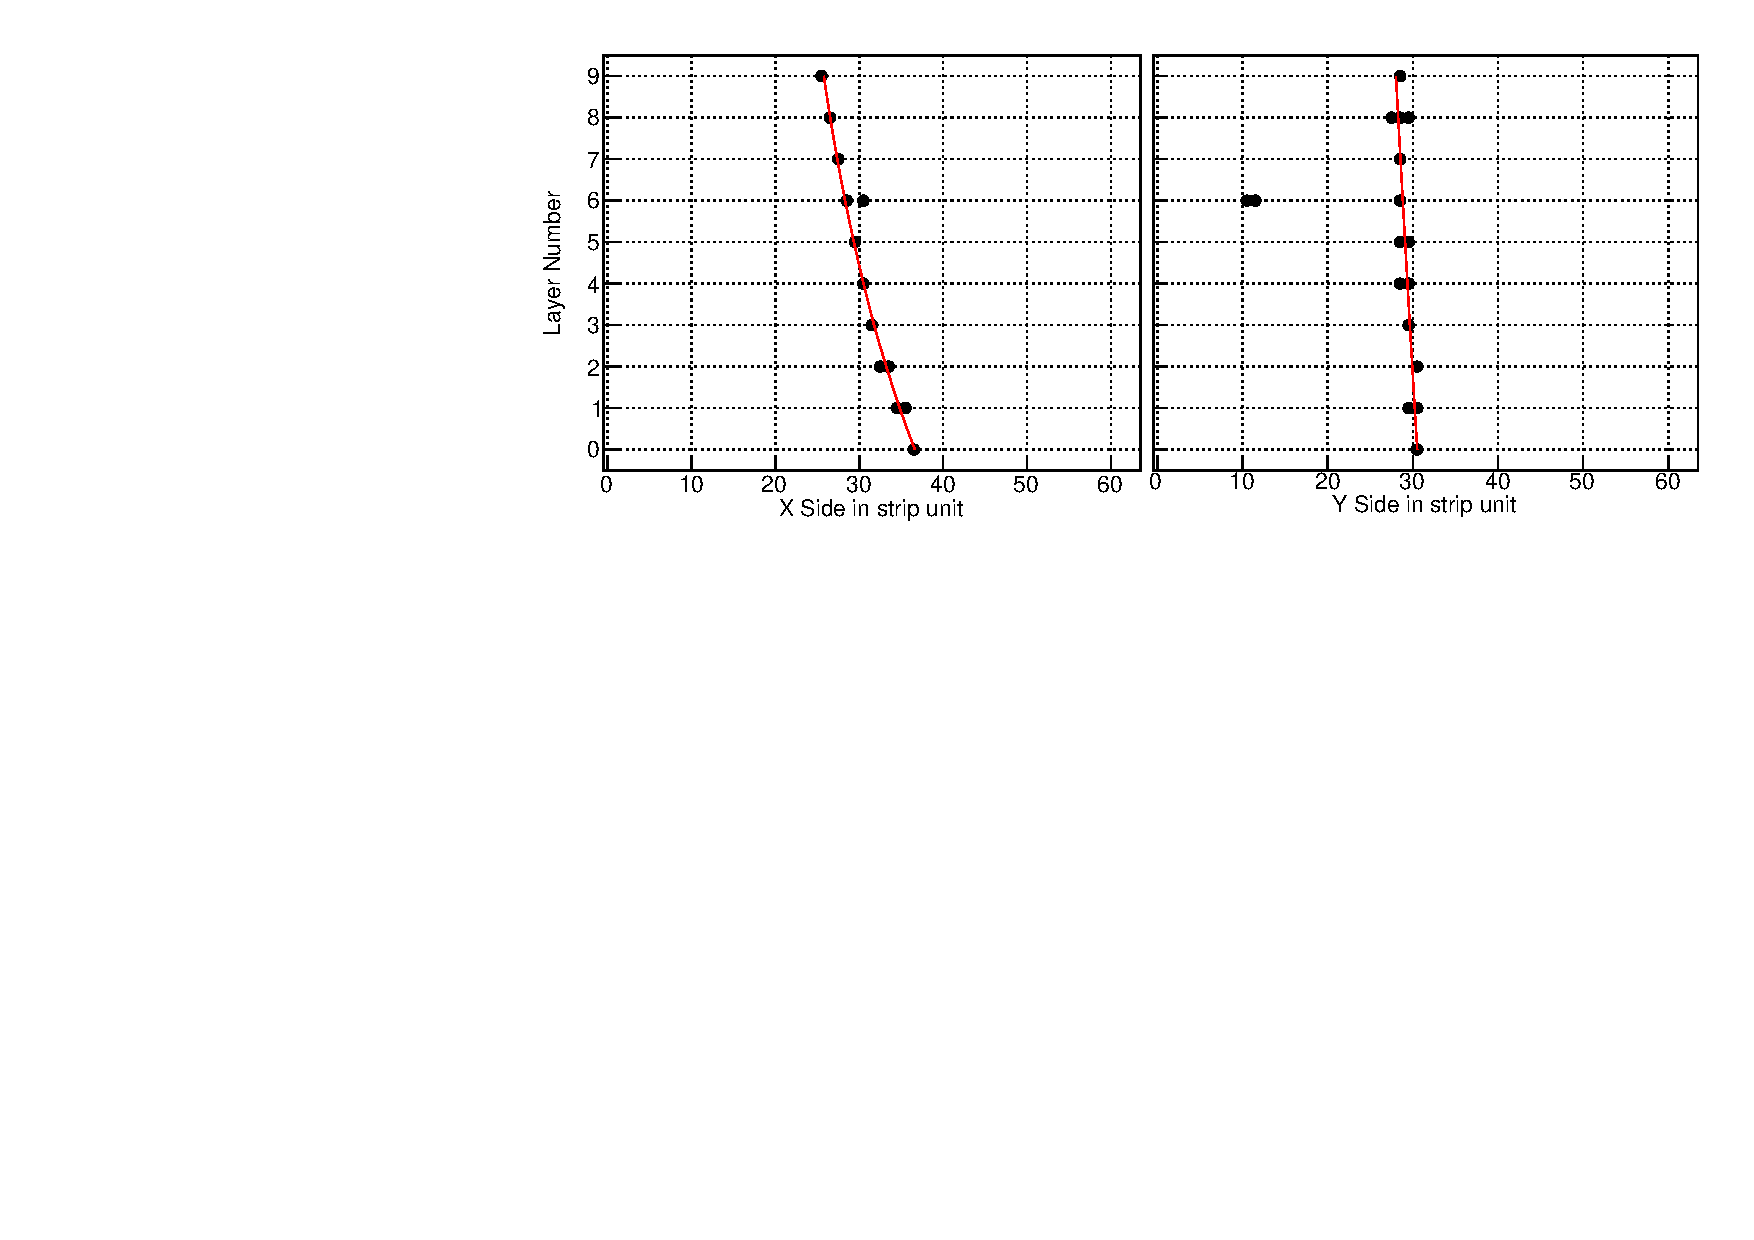
\includegraphics[width=1.0\linewidth]{Event_SNM_BRPCv4t_evtraw_20181212_091647_000045_1.pdf}
  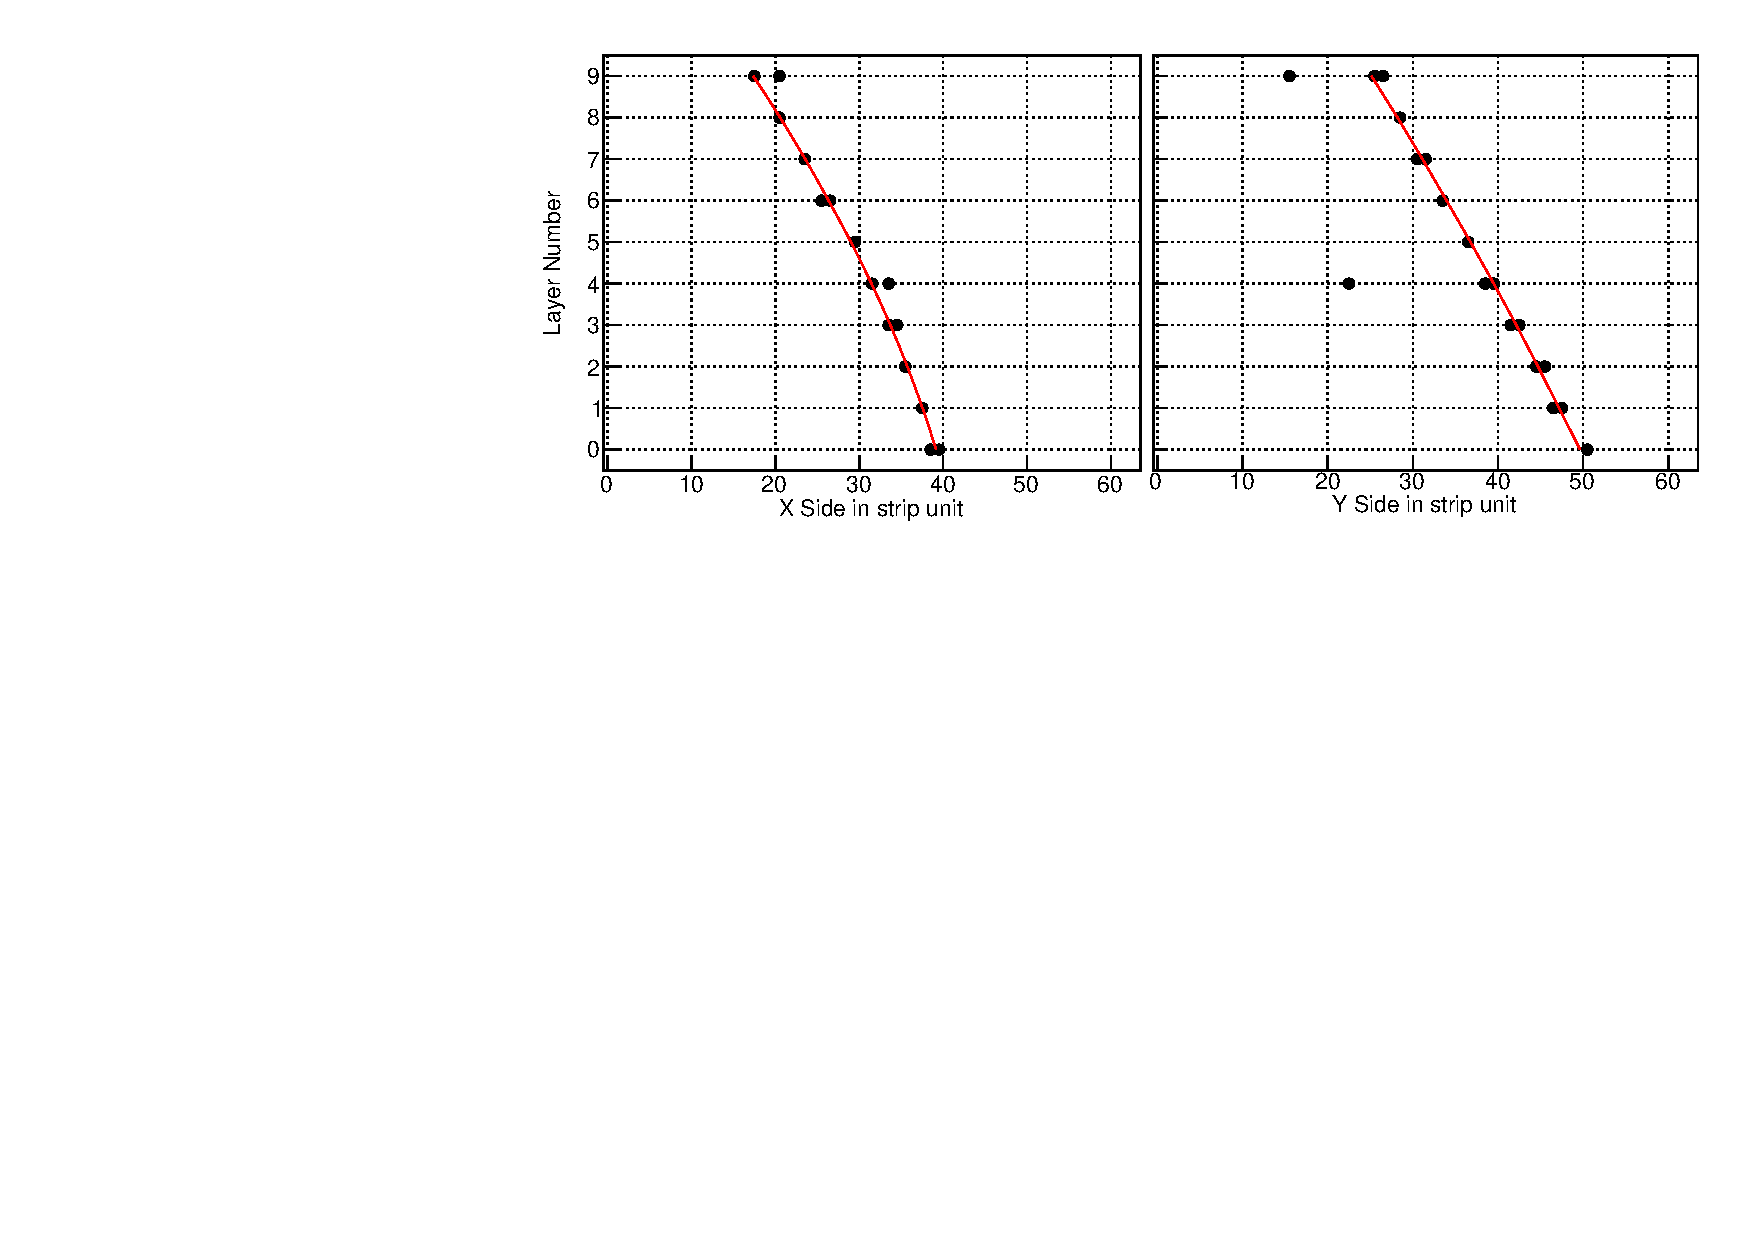
\includegraphics[width=1.0\linewidth]{Event_SNM_BRPCv4t_evtraw_20181212_091647_000157_1.pdf}
  \caption{Two events with reconstructed track with opposite charge.}
  \label{fig:eventdisplay}
\end{figure}

The clusters present in an event then are reconstructed using
different reconstruction algorithms to find the momentum of muons
which are discussed in the following.

\subsection{Circle Fit}
As it was shown earlier, the strength of the magnetic field in the
X-direction is very small. So, almost no significant bending is
observed in the Y-side of the track which makes the projection of
the track on the Y-side to be fit with a straight line.
Thus, in the first step of track reconstruction, the clusters on
the Y-side associated with the tracks are found and grouped using
the method of Hough Transformation\cite{hought}. This eliminates
the possibility of noise hits on the Y-side getting included in the
track reconstruction. Once one valid straight track is found, attention
is given on the X-side of the track. As the magnetic field is mainly
in the Y-direction, maximum bending of track is observed on the X-side.
The clusters on the X-side are then fitted with a circle.
The information of the fitted circle helps to reject the noise hits
on the X-side as well.
Using the radius ($r$ in meter) of the fitted circle, the transverse
momentum ($p_t$ in GeV) of the particle can be roughly estimated by
the following equation,
\begin{equation}
  p_{t}=0.3Br \label{eq:pt_est}
\end{equation}
where, $B$ is the average magnetic field in Tesla.

The information of the fitted straight line on the Y-side and the circle
on the X-side are further used to calculate the direction (zenith and
azimuth) of the incidence particle. From the direction and the $p_t$
value, the value of the momentum of the particle is estimated.

The events with muons are simulated using GEANT4. The hits obtained
at the GEANT4 simulation have been fitted using this method.
The estimated momentum vs the generated momentum is shown in the
Figure~\ref{fig:recomom}(a).
\begin{figure}[h]
  \centering
  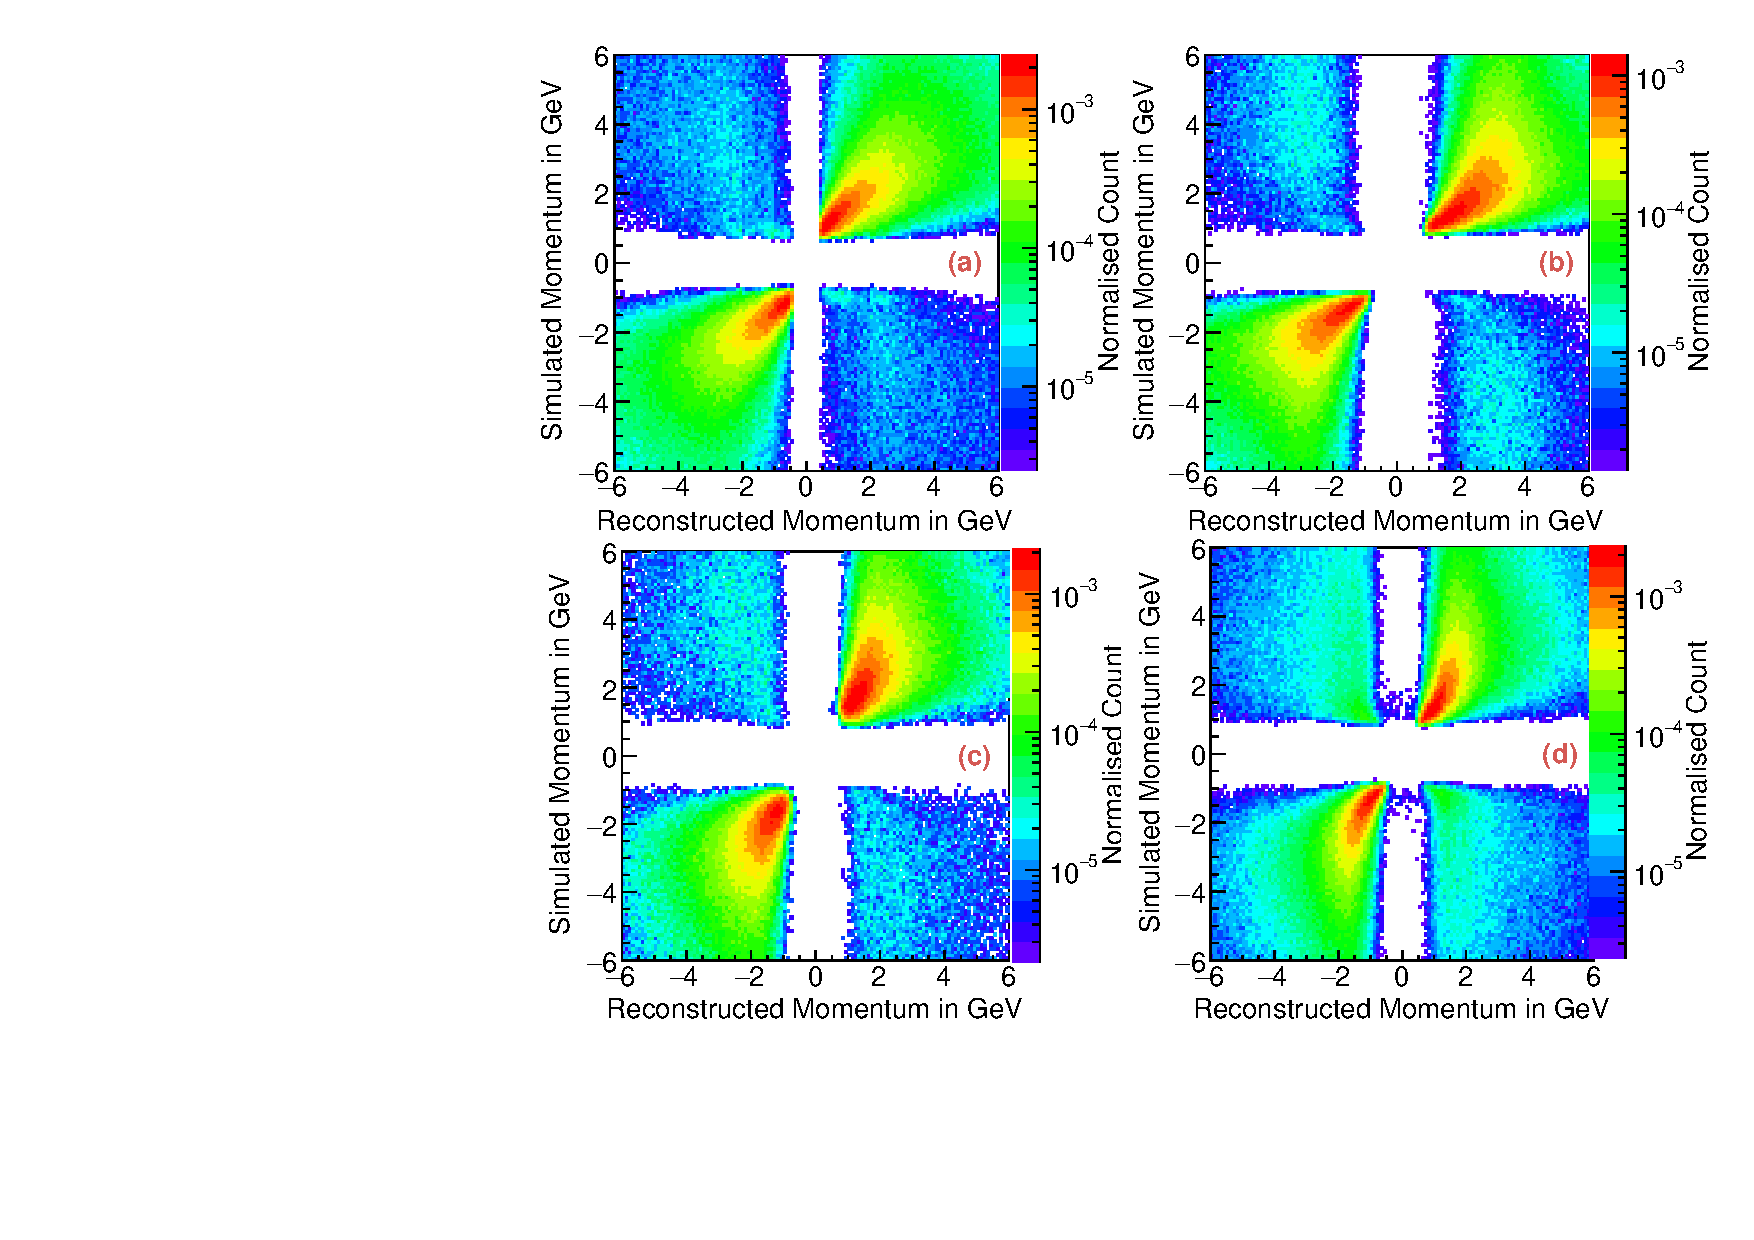
\includegraphics[width=0.9\linewidth]{responseMatrix_10Layer_All4.pdf}
  \caption{Generated momentum vs reconstructed momentum using
    (a) Circle Fit, (b) Grid-Search, (c) Explicit Track-Model
    and (d) Kalman-filter.}
  \label{fig:recomom}
\end{figure}


\subsection{Grid-Search Method}
The information from circle gives the rough estimate of the transverse
momentum ($p_{t}$) component of the momentum is calculated using the
radius of the circle. Combining the fit information from X-Z and Y-Z
plane, the track parameters i.e. two position and three momentum
components (such as $x,y,p_{x},p_{y},p_{z}$) are calculated. Whereas, the estimated
track parameters from above information can be well taken, if there
is no energy loss of the particles in detector medium and uniformity
of the magnetic field throughout the area. To get the correct values of
the track parameters, the energy loss of the material and the
non-uniformity in the magnetic field has to be taken care in the track
fitting.

To serve the purpose, the rough track parameters estimated from the
circle and straight line fit is fed as seed for the track
propagation, which is performed by solving the equation of motion of
charged particle in a magnetic field.

By using the $s$ as the free parameter, the equation of motion as given
by Lorentz force becomes,
\begin{equation}
  \frac{d^{2}{\bf r}}{ds^{2}}=\frac{q}{p}\frac{d{\bf r}}{ds}\,\times\,{\bf B(r)} = \lambda({\bf T}\,\times\,{\bf B(r)})~
  \label{eqn:lorentzeqn}
\end{equation}
where ${\bf T} = d{\bf r}/ds$ is the normalised tangent vector to the
track, ${\bf B(r)}$ is the magnetic field and $\lambda\sim q/p$. The
derivative $d{\bf r}/ds$ becomes $d{\bf r}/vdt = {\bf v}/v = {\bf T}$.

Analytical solution of the Eqn.~\ref{eqn:lorentzeqn} for a given
non-homogeneous magnetic field is impossible. Thus numerical solutions
are calculated. There are many numerical methods, among them one group
of methods used in tracking is Runge-Kutta Method. For this purpose,
the fourth order Runge-Kutta Nystrom \cite{lund2009track} method is
adapted.

The step size in the propagation is 3\,mm, which includes iron as well
as other material. After propagation, the measurement vector
$(x(z),y(z))$ are compared with predicted, where the propagation is done
using energy loss of muons in detector medium. The best fit parameters
$(x,y,p_{x},p_{y},p_{z})$ for an event is taken when the overall
$\chi^{2}$ for X- and Y-plane is minimum. This estimation is done by
varying the initial seed track parameters and then the particle is
propagated one by one and done for all five parameters.    

The hits obtained at the GEANT4 simulation have been reconstructed
using this method. The constructed momentum vs the generated momentum
is shown in the Figure~\ref{fig:recomom}(b).

\subsection{Explicit Track Model Fit}
The momentum was also reconstructed by the global track fitting using
the least-squares method (LSM) \cite{explicit1}. The track model is
the set of solutions of the equation of motion. The track model in the
LSM is the linear expansion of the function $f\left(p\right)$, where
$f$ is a deterministic function of the track parameter $p$. At a
reference surface, $p$ is defined by the $\left(x,y\right)$
coordinates and the momentum vector. As per the first approximation,
\begin{equation}
  f\left(p\right) = f\left(p_{0}\right) + A\cdot \left(p-p_{0}\right) + \mathcal{O} \left(p-p_{0}\right)^{2}+\cdots
\end{equation}
where $A=\frac{\partial f\left(p\right)}{\partial p}$ at $p=p_{0}$.

In the track model, the weight-matrix $W$ is defined as the inverse of
the covariance-matrix $V$. Since the measurement errors are
uncorrelated, then
\begin{equation}
  \left(W\right)_{ij} = \frac{\delta_{ij}}{\sigma_{j}^{2}}
\end{equation}
where $\sigma_{j}$ is the standard deviation on the $j^{\text{th}}$
measurement. But Generally, $W$ will have non-zero off-diagonal terms
in the case of multiple scatterings. During the track reconstruction,
the LSM tries to minimise the function,
\begin{equation}
  \chi^{2} = \left[f\left(p_{0}\right)+ A\cdot \left(p-p_{0}\right) - m\right]^{\mathrm{T}} \cdot W \cdot \left[f\left(p_{0}\right)+ A\cdot \left(p-p_{0}\right) - m\right]
\end{equation}

where,
\begin{description}
\item [$m = m(_i)$,] vector of measurements, e.g., $\theta, \phi$ (2$\times$N, number of track points)
\item [$f = (f_i)$,] vector of function corresponding to $m$, e.g., $\{x,y,dx/dz. dy/dz, q/p\}$
\item [$V$,] the covariance matrix of $m$, e.g., inverse of error matrices, (both position and effect of multiple scattering)
\item [$p_0$,] the approximate initial value of track parameters
\item [$A = \partial f/\partial p$,] at the point $p_0$
\end{description}

The solution of the least-squares problem,
\[p = p_0 + (A^T V^{-1} A)^{-1} A^T V ^{-1} (m -f(p_0))\]
and covariance matrix of $p$, $C(p) = (A^TV^{-1}A)^{-1}$.

The initial values of the track parameters are assigned to this fit
using a similar method discussed in the beginning of the Grid-Search.
The constructed momentum vs the generated momentum in the GEANT4 is
shown in the Figure~\ref{fig:recomom}(c).


\subsection{Kalman-Filter Fit}
This reconstruction method is a Kalman-filter based algorithm, where
every track is initiated by a state vector
$X_{0}=\left(X,Y,dX/dZ,dY/dZ,q/p\right)$. The state vector contains
the position of the starting hit $\left(X,Y,Z\right)$,
the charge-weighted inverse momentum which is taken to be zero and
the initial direction (the slopes $dX/dZ$, $dY/dZ$) which is
estimated from the first two layers. The initial state vector is then
extrapolated to the next layer using an extrapolation algorithm based
upon the equation of motion of a particle in a magnetic field. The
extrapolated state vector is then filtered and improved using the
Kalman-filter based algorithm. In this algorithm, the corresponding
error propagation is predicted by a propagation matrix \cite{kalman1}.
The Kalman-filter also takes the process of the multiple-scattering
as described in \cite{kalman2} and the energy loss in matter according
to the Bethe formula \cite{bethe1}. The extrapolated point is then
judged with the actual position of the hit in that layer, if any, and
the process is iterated. The best fit track is obtained from the
complete iteration. The $q/p$ determines the magnitude of the momentum
along with the reconstructed direction using $dX/dZ$ and $dY/dZ$, which
are the zenith and azimuth angles respectively.

In short, State vector at any step is the combination of extrapolation from previous
measurement and measurement at that point,
$$  p^k_k = K^1_k \,p^{k-1}_k + K^2_k \,m_k, \hspace{2cm} p_k^{k-1} = F_{k-1}\,p_{k-1}$$
where,  $K^1_k$ and $K^2_k$ are two weight factors, $p^{k-1}_k$ is the expected state
vector from previous measurements. The weight factors is calculated
(for true state vector, $p$) from the minimisation of
$$\chi^2  = (m_k - f(p))^T \,V^{-1}\, (m_k - f(p)) + (p - p_k^{k-1})^T \,(C^{k-1}_k)^{-1} \,(p - p_k^{k-1})$$

which has the following matrix algebra for each step
\begin{eqnarray*}
  V &=& (V_k + A_k \,C_k^{k-1} \,A_k^T) \\
  C^{k-1}_k &=& F_{k-1}\, C_{k-1}\, F^T_{k-1} + Q_{k-1} \\
  K_k &=& C^{k-1}_k\, A_k^T (V_k + A_k\, C^{k-1}_k\, A_k^T)^{-1} \\
  p_k &=& F_{k-1}\, p_{k-1} + K_k (m_k - A_k \,F_{k-1}\,p_{k-1}) \\
  p_k &=& (I-K_k\,A_k)\, p_k^{k-1} + K_k\;m_k \\
  C_k &=& (I - K_k\, A_k)\, C_k^{k-1} \\
\end{eqnarray*}

where,
\begin{itemize}
\item $p_k$ : State vector $ \{x, y, dx/dz, dy/dz, q/p\}$, ($5 \times 1$)
\item $C_k$ : State covariance matrix, ($5 \times 5$)
\item $F_k$ : Propagator matrix of state vector $p_k$, ($5 \times 5$)
\item $Q_k$ : Noise matrix due to multiple scattering/ionisation loss, ($5 \times5) $
\item $m_k$ : X(Y) position measurement, ($2 \times 1$)
\item $V_k$ : Error matrix of $m_k$, ($2 \times 2$)
\item $A_k$ : Measurement function ($\partial f /\partial p_k$ from experiment $m_k=f(p_k)$), ( $2 \times 5$)
\item $K_k$ :  Kalman gain factor, ($5 \times 2$)  \\
  $K^1_k = (I - K_k\,A_k)$ and $K^2_k = K_k$
\end{itemize}  

The hits obtained from the GEANT4 simulation are reconstructed using
this method. The constructed momentum vs the generated momentum is
shown in the Figure~\ref{fig:recomom}(d).



\section{Charge Ratio Spectra of Cosmic Ray Muons}
\label{section:multiresult}

It can be observed in the Figure~\ref{fig:recomom} that the particles
with momentum less than 0.8\,GeV are not reconstructed. This is because
of the minimum momentum cutoff due to the minimum layer criteria of 7.
Also the insignificant curvature of the tracks at higher momentum
coupled with the strip width of the pickup panels, constrains the
reconstruction for larger momentum.

In order to compare the the fit methods quantitatively, the Mean and
RMS of the $\left(P_{reco}-P_{gen}\right)$ plot is calculated for
different interval of $P_{gen}$ values, which is shown in the
Figure~\ref{fig:meanrms}.
\begin{figure}[h]
  \centering
  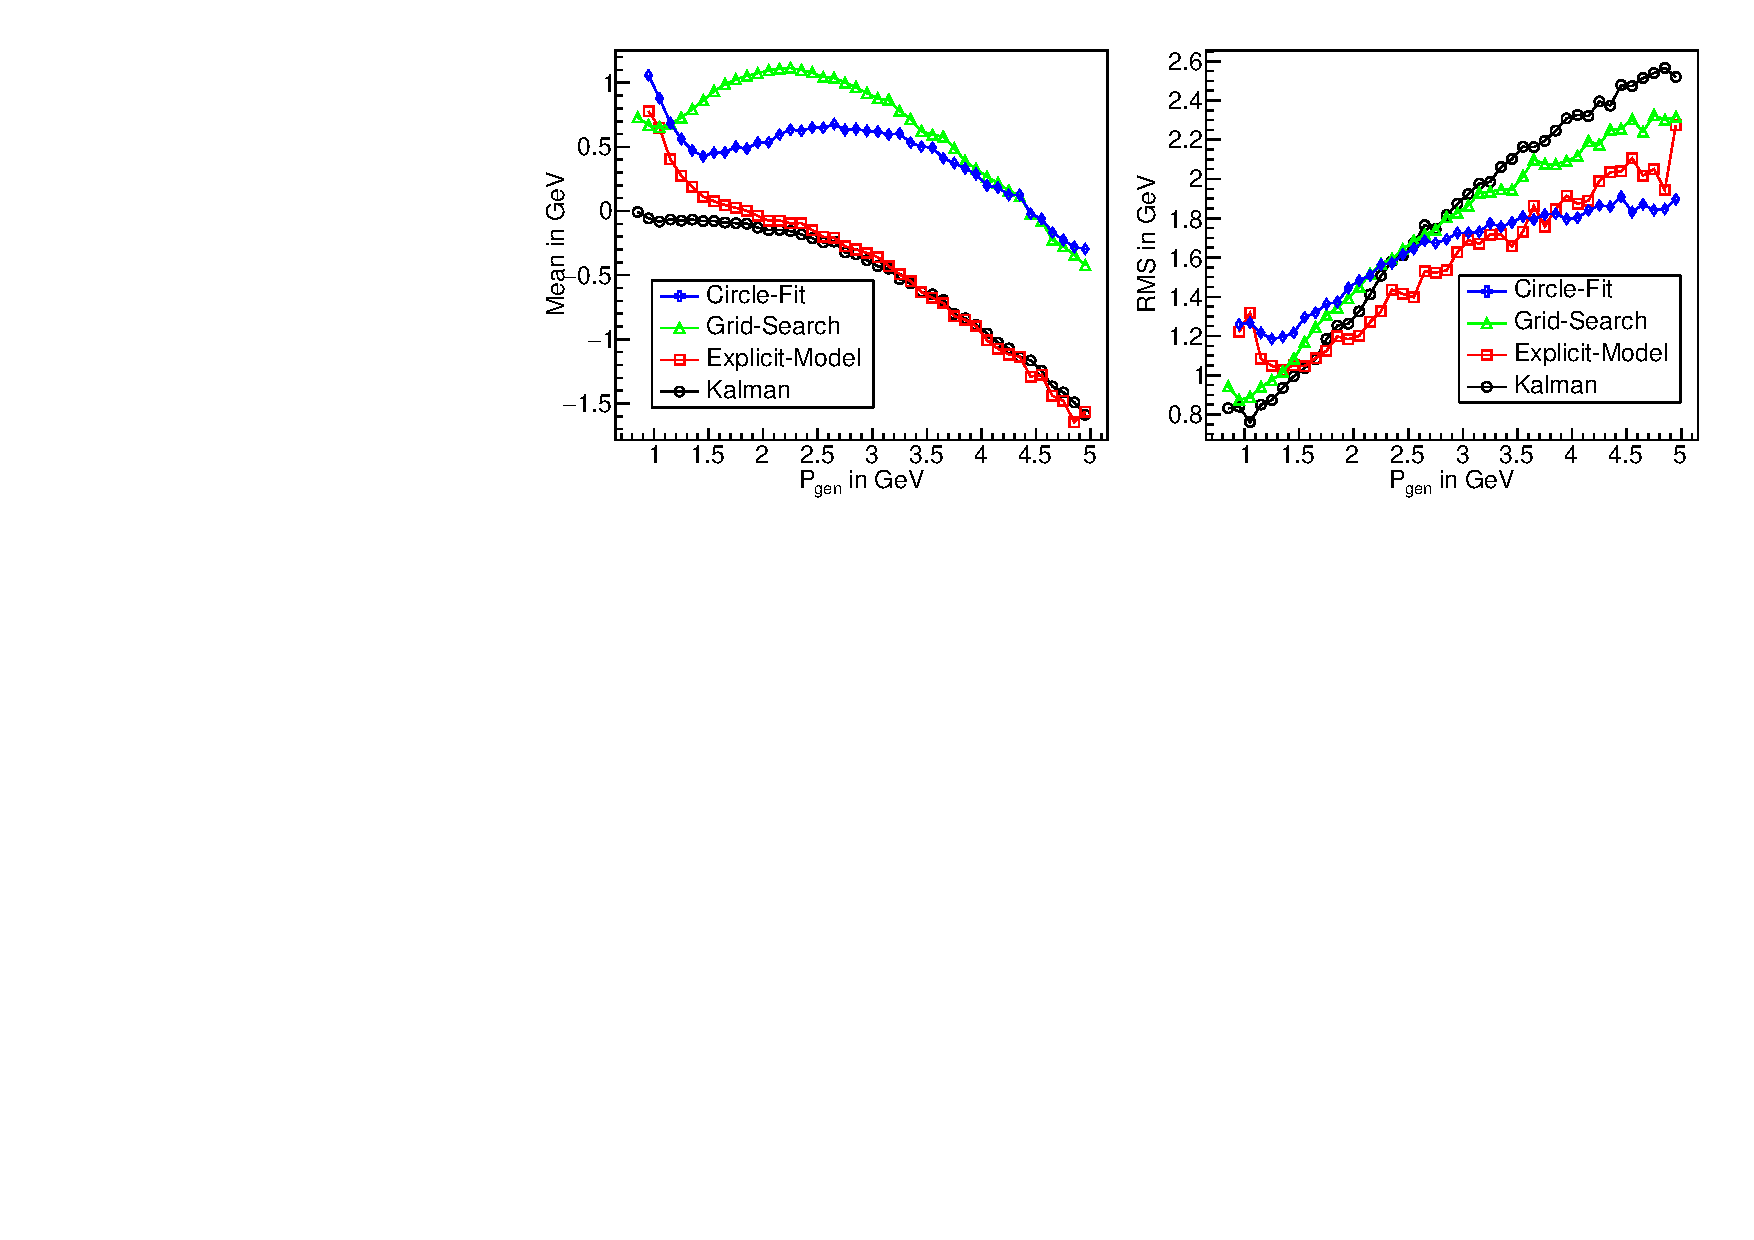
\includegraphics[width=0.8\linewidth]{GMA_mean_rms_All4.pdf}
  \caption{the Mean and RMS of the $\left(P_{reco}-P_{gen}\right)$ plot
    for different values of $P_{gen}$.}
  \label{fig:meanrms}
\end{figure}
It is clear from plots in \ref{fig:recomom} that Kalman filter techniques shows
a saturation of reconstructed momentum at around 2\,GeV, which is mainly due to
the large uncertainty in position measurement and limited number of measured points.
That is true to some extent for the explicit Track-Model also. Due to the saturation
of magnetic field, there is a gradual shifts in mean of  $\left(P_{reco}-P_{gen}\right)$
for these two cases. The circle fit has a bias mainly due to ionisation energy loss, which
was not incorporated there. Apparent bias in Grid Search techniques is mainly due to
momentum ranges in generated MC samples. But, there is almost no difference in RMS in
those four fitting techniques due to larger tails in the distributions.

The $\left(P_{reco}-P_{gen}\right)$ plots for different intervals of
$P_{gen}$ are also fitted with {\it Landau} function. The maximum
probable value (MPV) and $\sigma$ of the plots are shown in the
Figure~\ref{fig:mpvsigma}.
\begin{figure}[h]
  \centering
  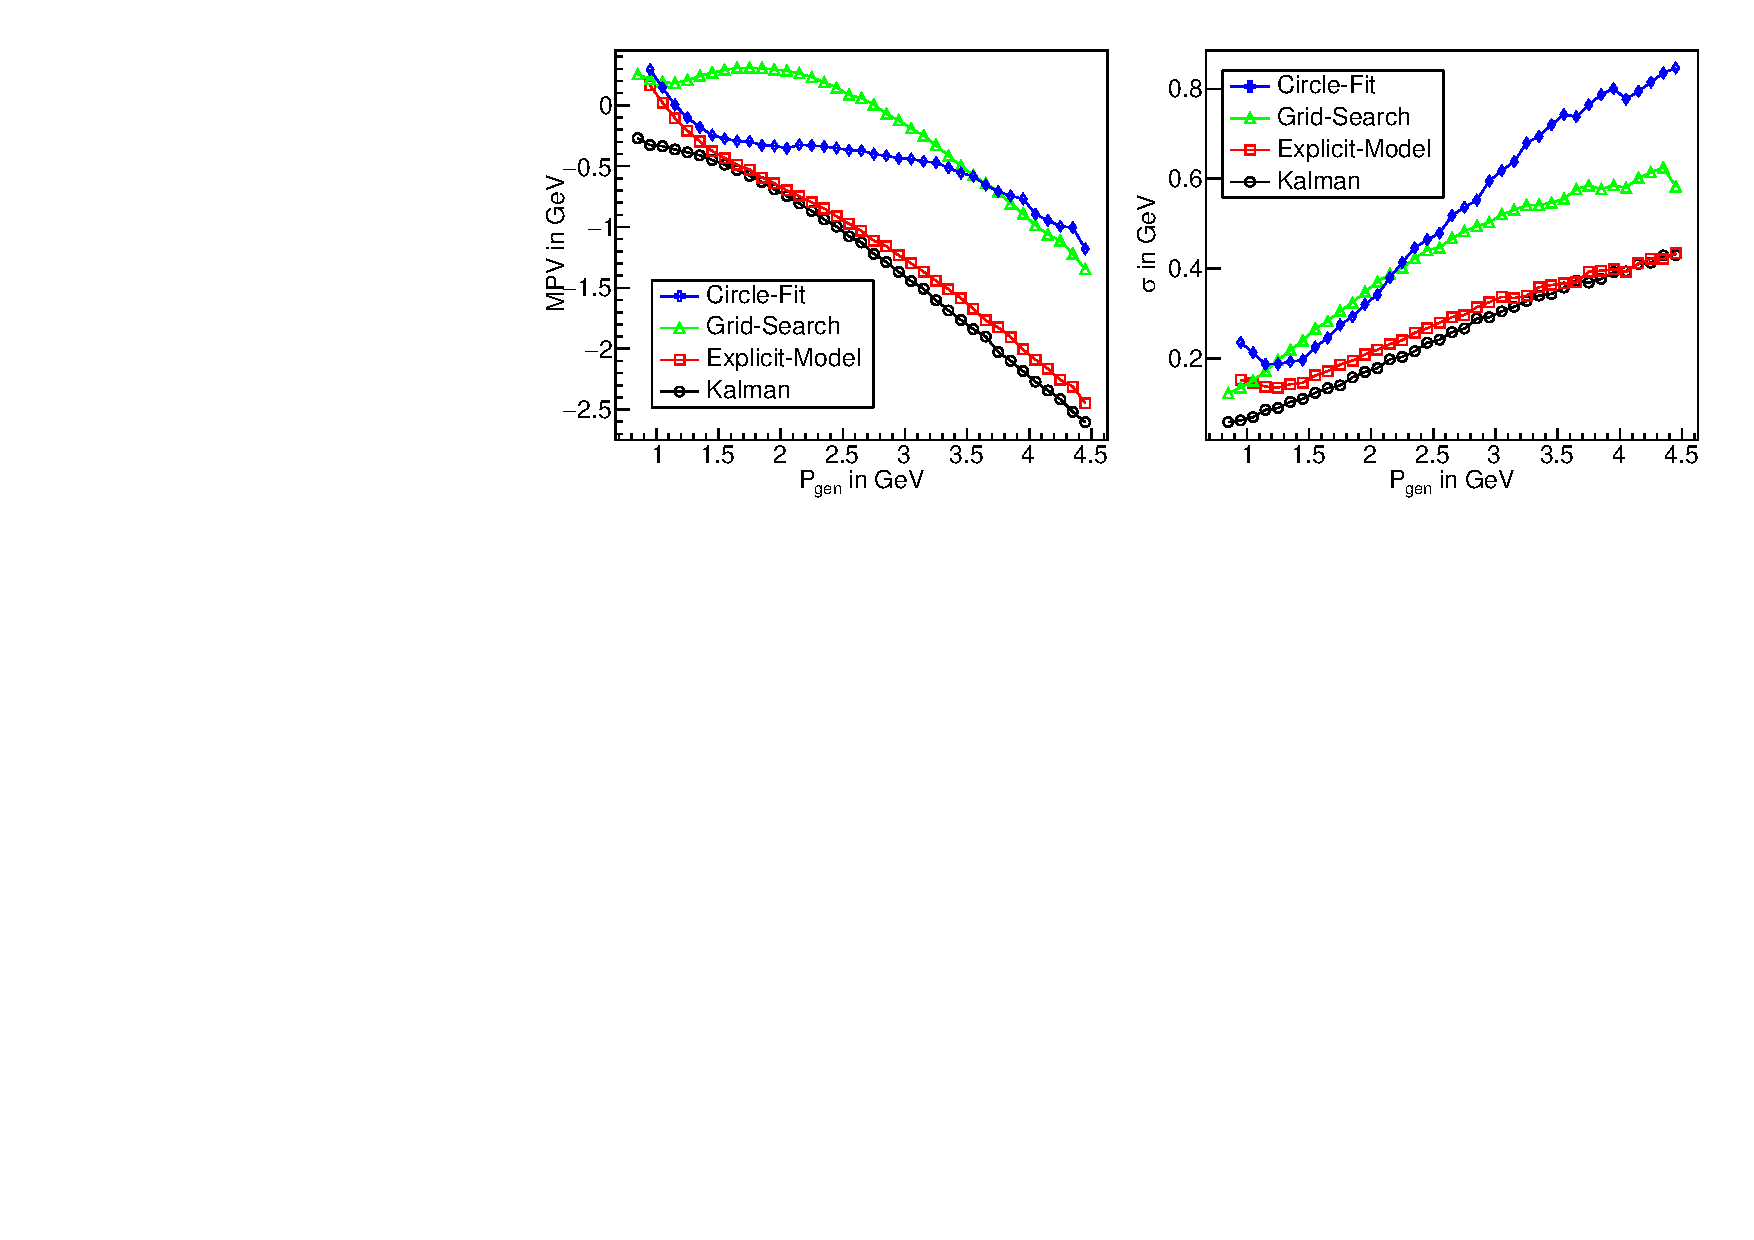
\includegraphics[width=0.8\linewidth]{GMA_mpv_sigma_All4.pdf}
  \caption{The MPV and $\sigma$ of the $\left(P_{reco}-P_{gen}\right)$
    plot for different values of $P_{gen}$.}
  \label{fig:mpvsigma}
\end{figure}
In the fitted $\mu$ (\ref{fig:mpvsigma}(b)), the same bias is there for Kalman fit
and explicit track fit models, whereas due to less effect of tails part, bias in
the grid search model has reduced drastically. The apparent better $\sigma$ in
the \ref{fig:mpvsigma}(b) from Kalman fit and explicit track fit models are due to
saturation effects, which is really not a good resolution.

Each model also has its limitation in the efficiency and the capacity of
determining the charge of the particle. The efficiency is defined as
the ratio between the number of particles reconstructed to that of
particles generated provided the charge of the particles are identified
properly. The efficiency of the fit methods are shown in the
Figure~\ref{fig:miseffi}(a).
The amount of mis-identification of the charge of a particle
is represented in the Figure~\ref{fig:miseffi}(b).
\begin{figure}[h]
  \centering
  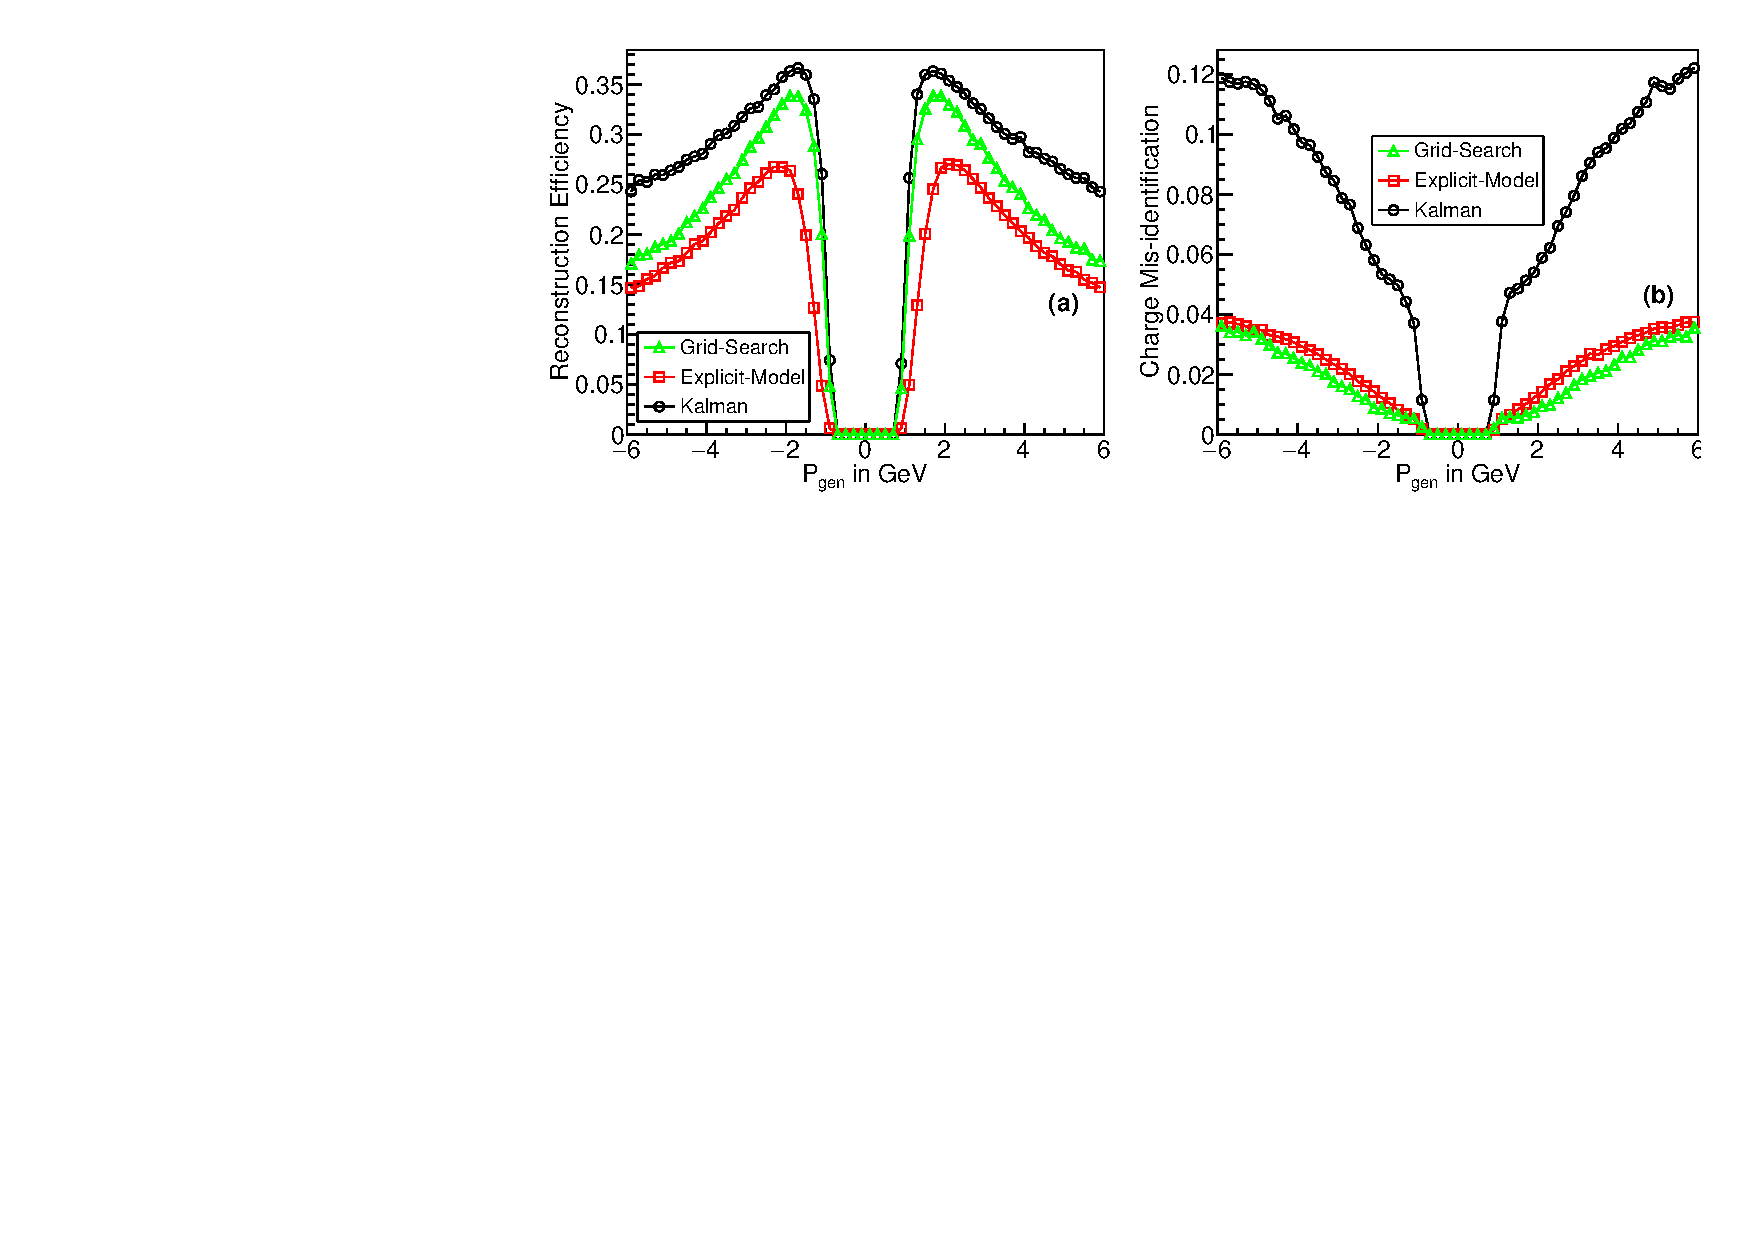
\includegraphics[width=0.8\linewidth]{GMA_effi_misId_All3.pdf}
  \caption{(a) Efficiency of the fit methods and (b) Particle charge
    mis-identification plotted against $P_{gen}$.}
  \label{fig:miseffi}
\end{figure}

%% The limitations of the fit-methods described above is now discussed
%% in the following.
%% %% \vspace*{-10pt}
%% \begin{itemize} %% \itemsep -5pt
%% \item Though the Kalman-filter shows better momentum resolution at
%%   lower momentum, the reconstructed momentum saturates beyond
%%   $\sim$1.6\,GeV. The mis-identification of the charge of the particles
%%   is also large in this fit method as it starts the reconstruction
%%   with $q/p=0$.
%% \item Explicit Track-Model fit shows slightly poorer resolution for the
%%   reconstruction of muon trajectories than the Kalman-filter.
%%   But it performs better than the Kalman-Filter in terms of saturation
%%   of reconstructed momentum. The mis-identification is less than the
%%   Kalman-Filter as this method determines the charges of the particles
%%   from the direction of the curvature of the particles.
%% \item Though the method of Grid-Search performs better in terms of
%%   the saturation of reconstructed momentum as well as its momentum resolution
%%   in comparison with other three models. The charge mis-identification
%%   is less as this method also indicates the capabilities of better momentum
%%   measurement.
%% \end{itemize}

Taking the performance of the fit methods on the basis of charge
mis-identification, overall momentum resolution and saturation of
reconstructed momentum; the Grid Search Method has been
accepted to further study the charge ratio of the cosmic ray muons.

The measured momentum spectra in the detector is biased
because of the housing building covering the detector, limited
acceptance of the detector, resolution and other systematic effects
on the detector. This can be represented by the following equation,
\begin{equation}
  {\bf A}{\bf x}+{\bf b}={\bf y}
  \label{eq:unfold}
\end{equation}
where, {\bf A} is the `response matrix', {\bf x} is the `truth' spectra,
{\bf b} is the `background' and {\bf y} is the `measured' spectra.
The procedure of estimating the {\it truth} spectra using known
{\it response matrix} and {\it background} spectra is called
data-unfolding. So to compare the experimental measurement with
previous prediction, the reconstructed spectra is unfolded to eliminate
the detector's effects.
The unfolding method used for the current
study is iterative Bayesian Unfolding \cite{bayesian}.

In order to determine the number of iterations required in the
unfolding process, the following procedures have been adopted.
\begin{itemize} %% \itemsep -5pt
\item The MPV and $\sigma$, found in the case of Grid Search method
  (shown in the Figure~\ref{fig:mpvsigma}), are used to smear
  the randomly generated momentum values. The generated and smeared
  values of the momentum are then filled in a histogram to create
  the response matrix, which is shown in the
  Figure~\ref{fig:unfolditer}(a).
\item The above step is then repeated again with different seed,
  but for this time to create the spectra to be unfolded. The spectra
  created using randomly generated momentum value is the {\it truth},
  and the spectra created by using the smeared momentum is the
  {\it measured}.
\item The {\it measured} spectra created in the previous step is then
  unfolded using the iterative Bayesian technique for different numbers
  of iterations. The unfolded spectra is then compared with the
  {\it truth}. The difference between the unfolded spectra and the
  {\it truth}, termed as $\chi^{2}$, is plotted against the number of
  iterations which are shown in the Figure~\ref{fig:unfolditer}(b).
  It can be seen that the unfolding is minimised at iteration number 4.
\end{itemize}
\begin{figure}[h]
  \centering
  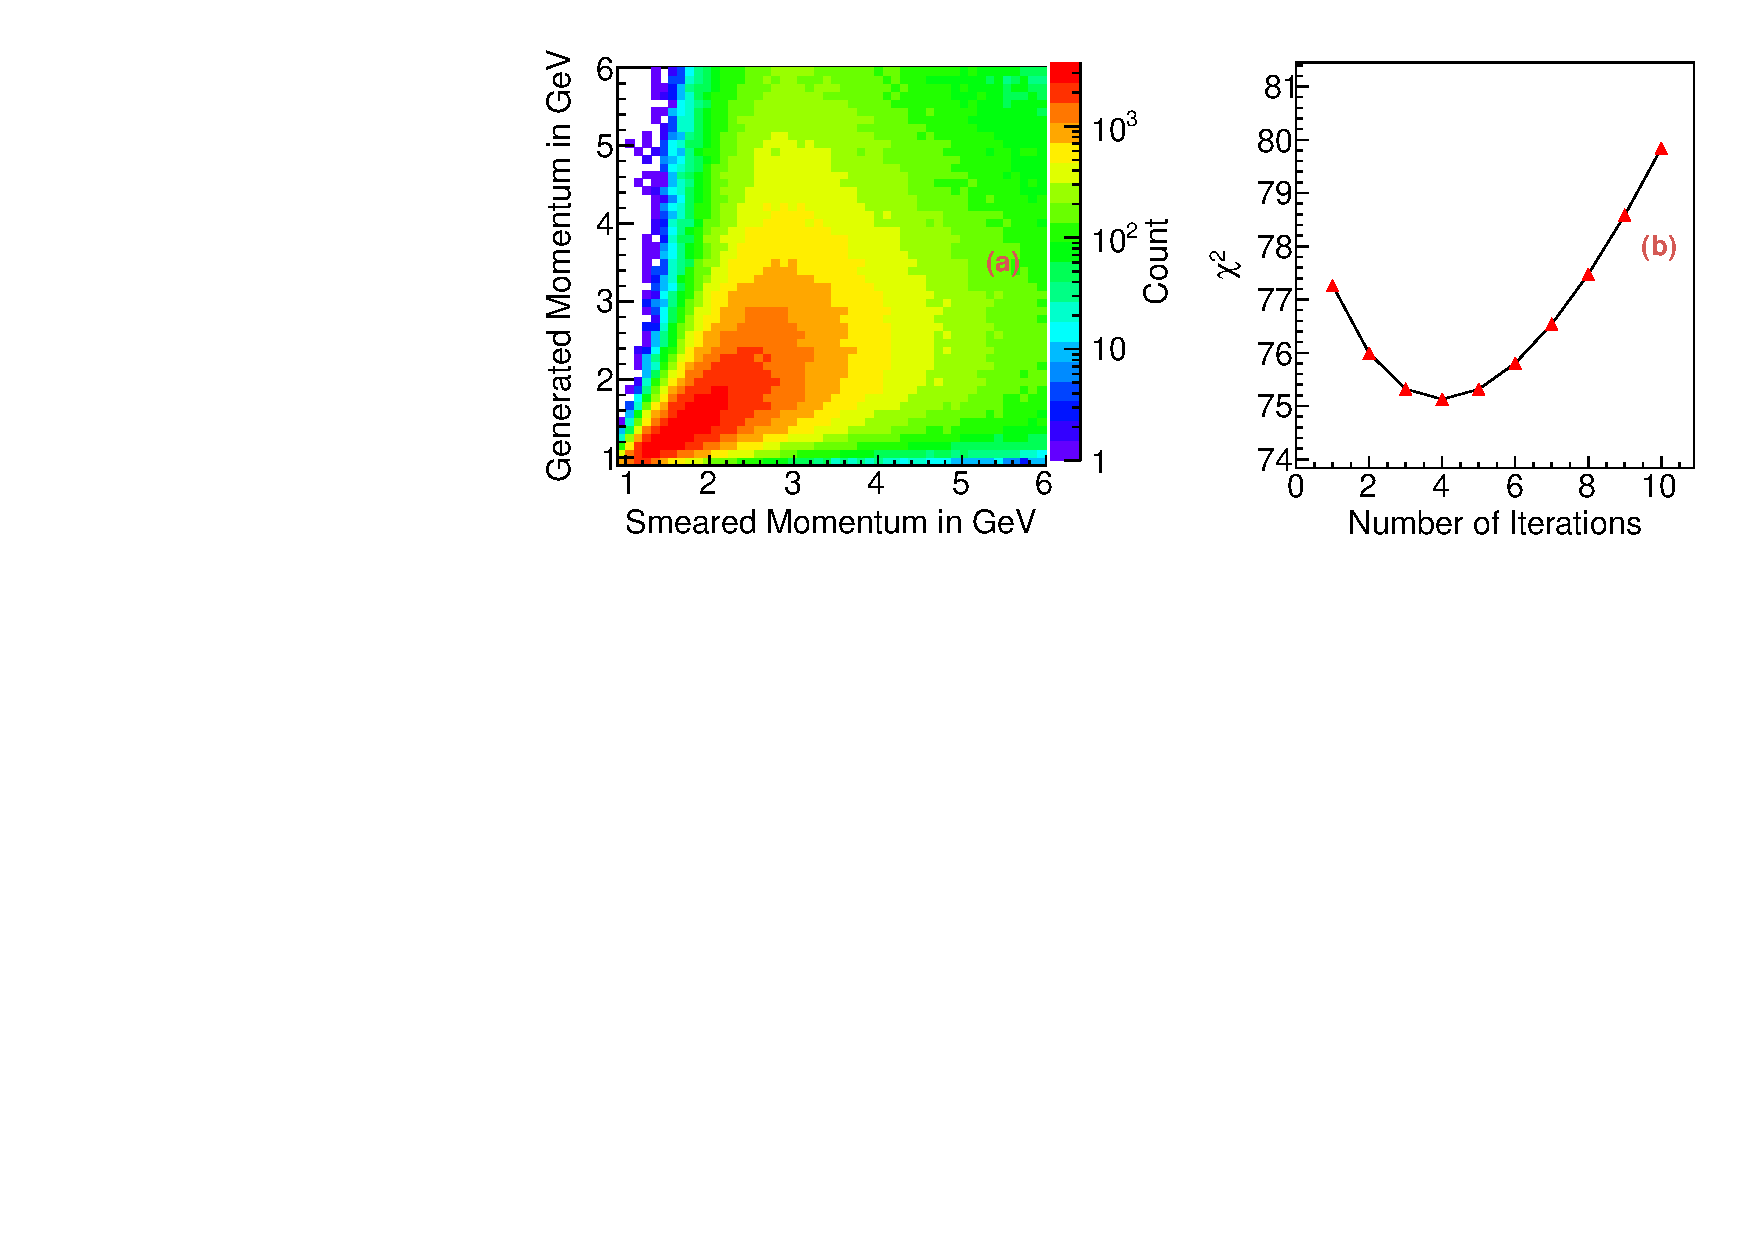
\includegraphics[width=0.8\textwidth]{ResoResponse_Grid.pdf}
  \caption{(a) Generated Response Matrix and
    (b) $\chi^{2}$ vs Number of Iteration.}
  \label{fig:unfolditer}
\end{figure}

The cosmic ray events collected in the mini-ICAL detector are
constructed using the Grid search method. The reconstructed momentum
spectra is then unfolded using the response matrix calculated from
GEANT4 simulation (shown in the Figure~\ref{fig:recomom}(c)).
In the Bayesian technique, the background in each reconstructed
momentum bin and efficiency of each true momentum bin are calculated.
The reconstructed data and MC are also corrected for fake rate.
The unfolded momentum spectra for $\mu^{+}$ and $\mu^{-}$ is shown in
the Figure~\ref{fig:unfolddata}(a).
The charge ratio $(R)$ of the atmospheric muons is then found by
dividing the spectra for $\mu^{+}$ with the spectra for $\mu^{-}$,
which is shown in the Figure~\ref{fig:unfolddata}(b).
\begin{figure}[h]
  \centering
  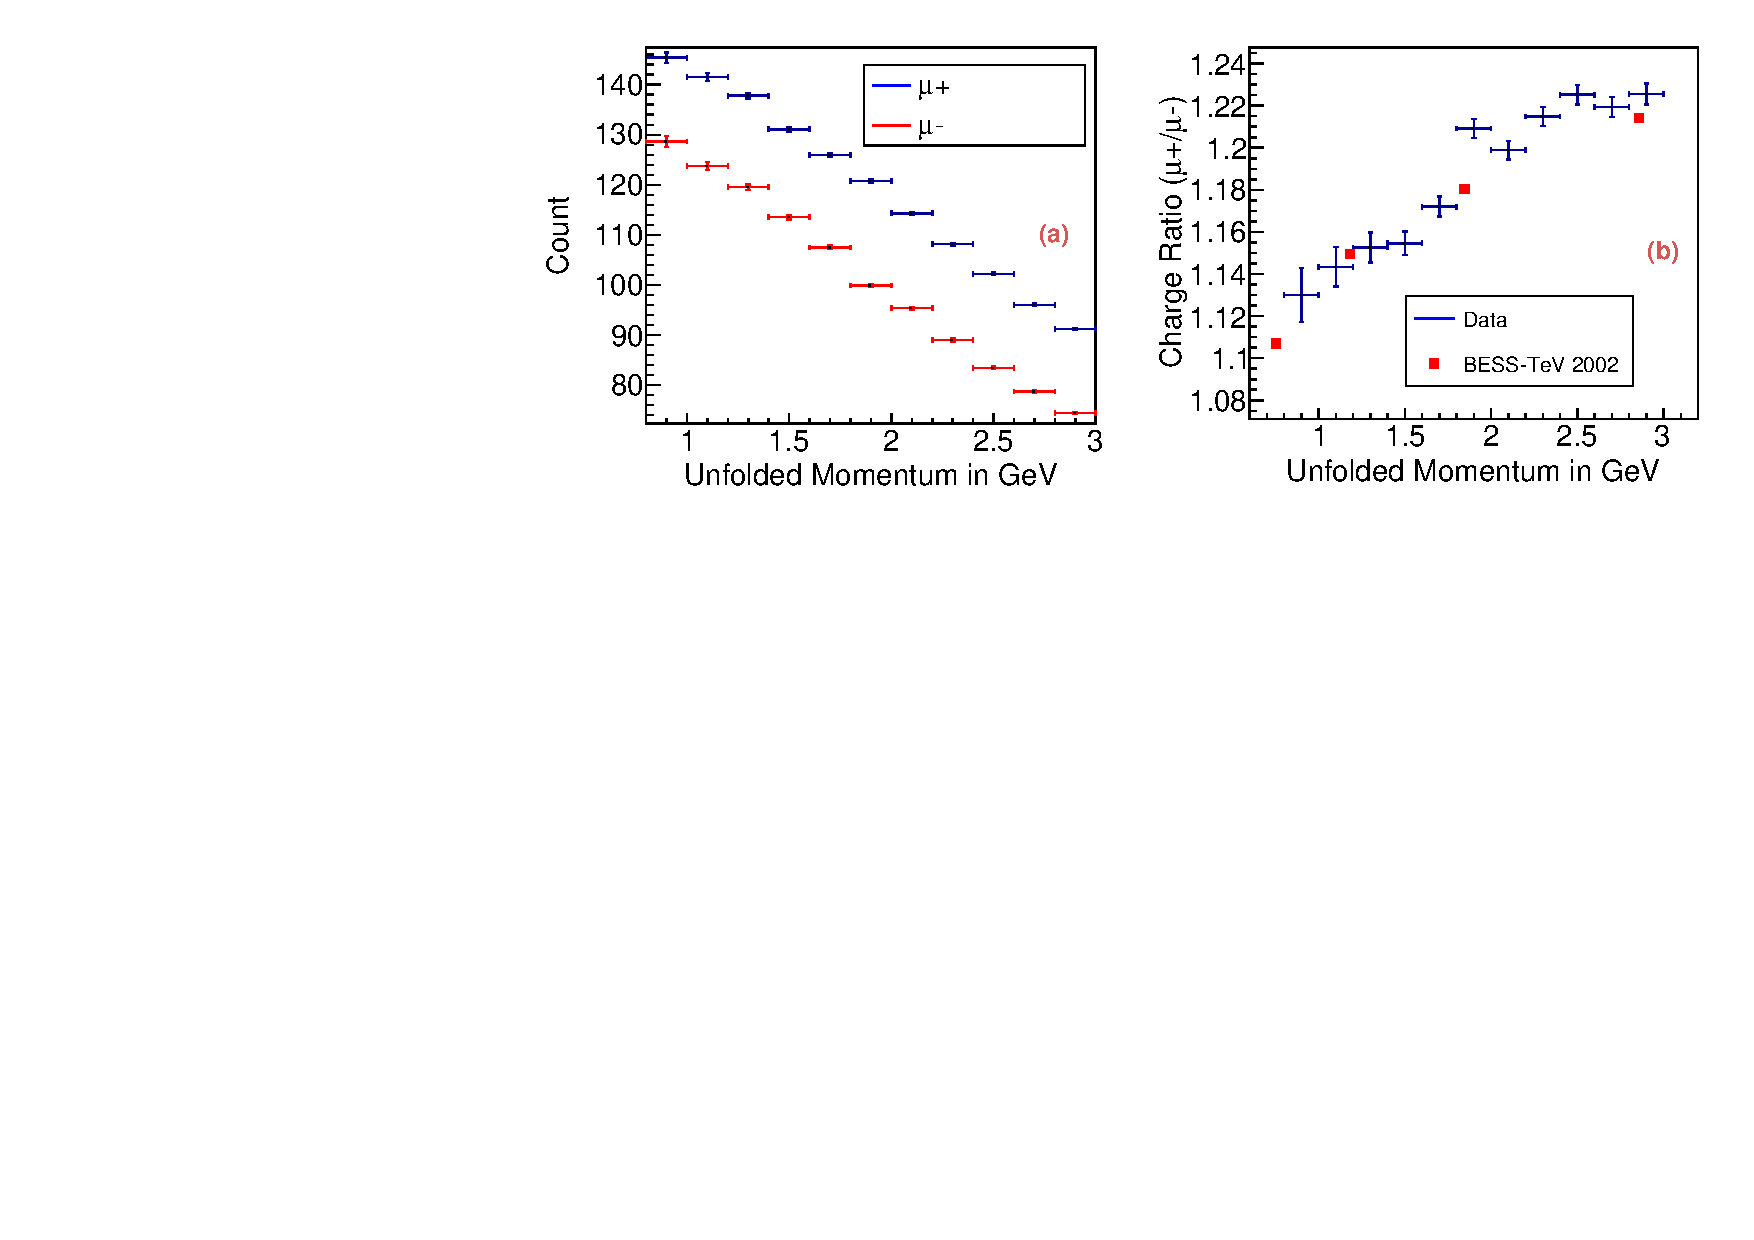
\includegraphics[width=0.8\linewidth]{UnfoldedPlot_Grid.pdf}
  \caption{(a) Unfolded momentum spectra for $\mu^{+}$ and $\mu^{-}$
    reconstructed from data, (b) Charge ratio of muons compared
    with BESS-TeV'02 calculation \cite{bess2002}.}
  \label{fig:unfolddata}
\end{figure}

The reconstructed spectra from data are unfolded up-to 3\,GeV as the
reconstructed energy saturates beyond this energy \cite{daeratio,ratio1}. %GMA, put the reference of DAE talk and also add another citation "Muon charge ratio at Madurai, S. Mondal, S. Pethuraj, G. Majumder" in preparation.
A new detector setup, named as Engineering Module is going to be
built in the near future. This setup is going to have 20 layers of RPC
detectors.
\begin{figure}[h]
  \centering
  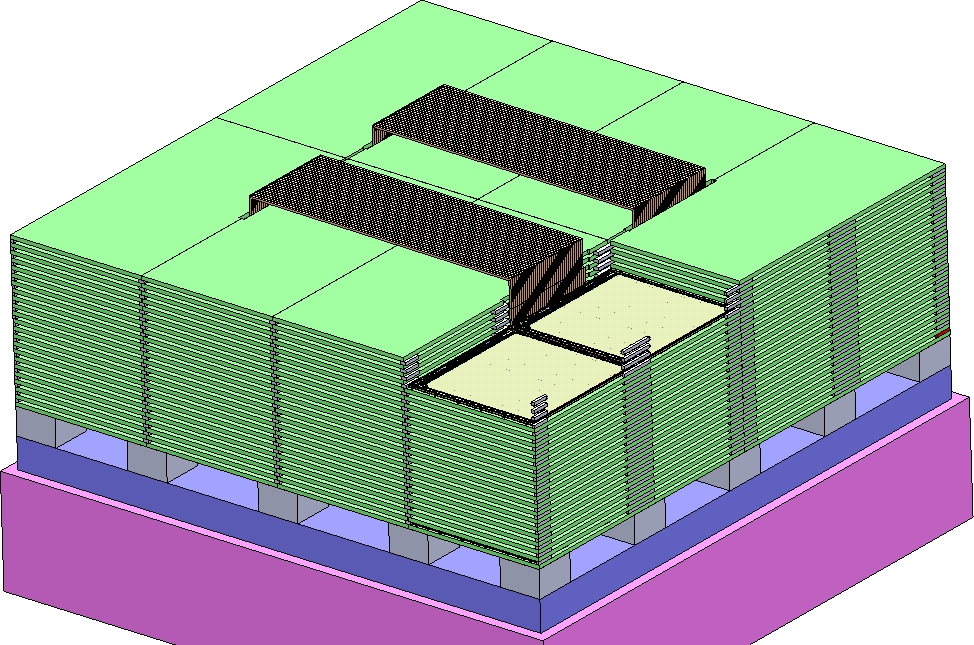
\includegraphics[width=0.75\linewidth]{engMod.png}
  \caption{Model of the Engineering Module.}
  \label{fig:eng_mod}
\end{figure}
The Grid Search method is giving better results for a 10 layer setup, but it is taking too
much time to simulate it. Also, is it expected that with larger hit points, explicit
track fit model will give better resolution. Thus to reduce the reconstruction time
explicit track fit model is used to reconstruct muons at 20 layers Engineering module.
A preliminary simulation is performed with this setup by assuming the
position of the RPCs in the central region of the detector. The events
with more than 14 layer of hits are reconstructed.
The response matrix found from this simulation is shown in the
Figure~\ref{fig:eng_mod}.
\begin{figure}[h]
  \centering
  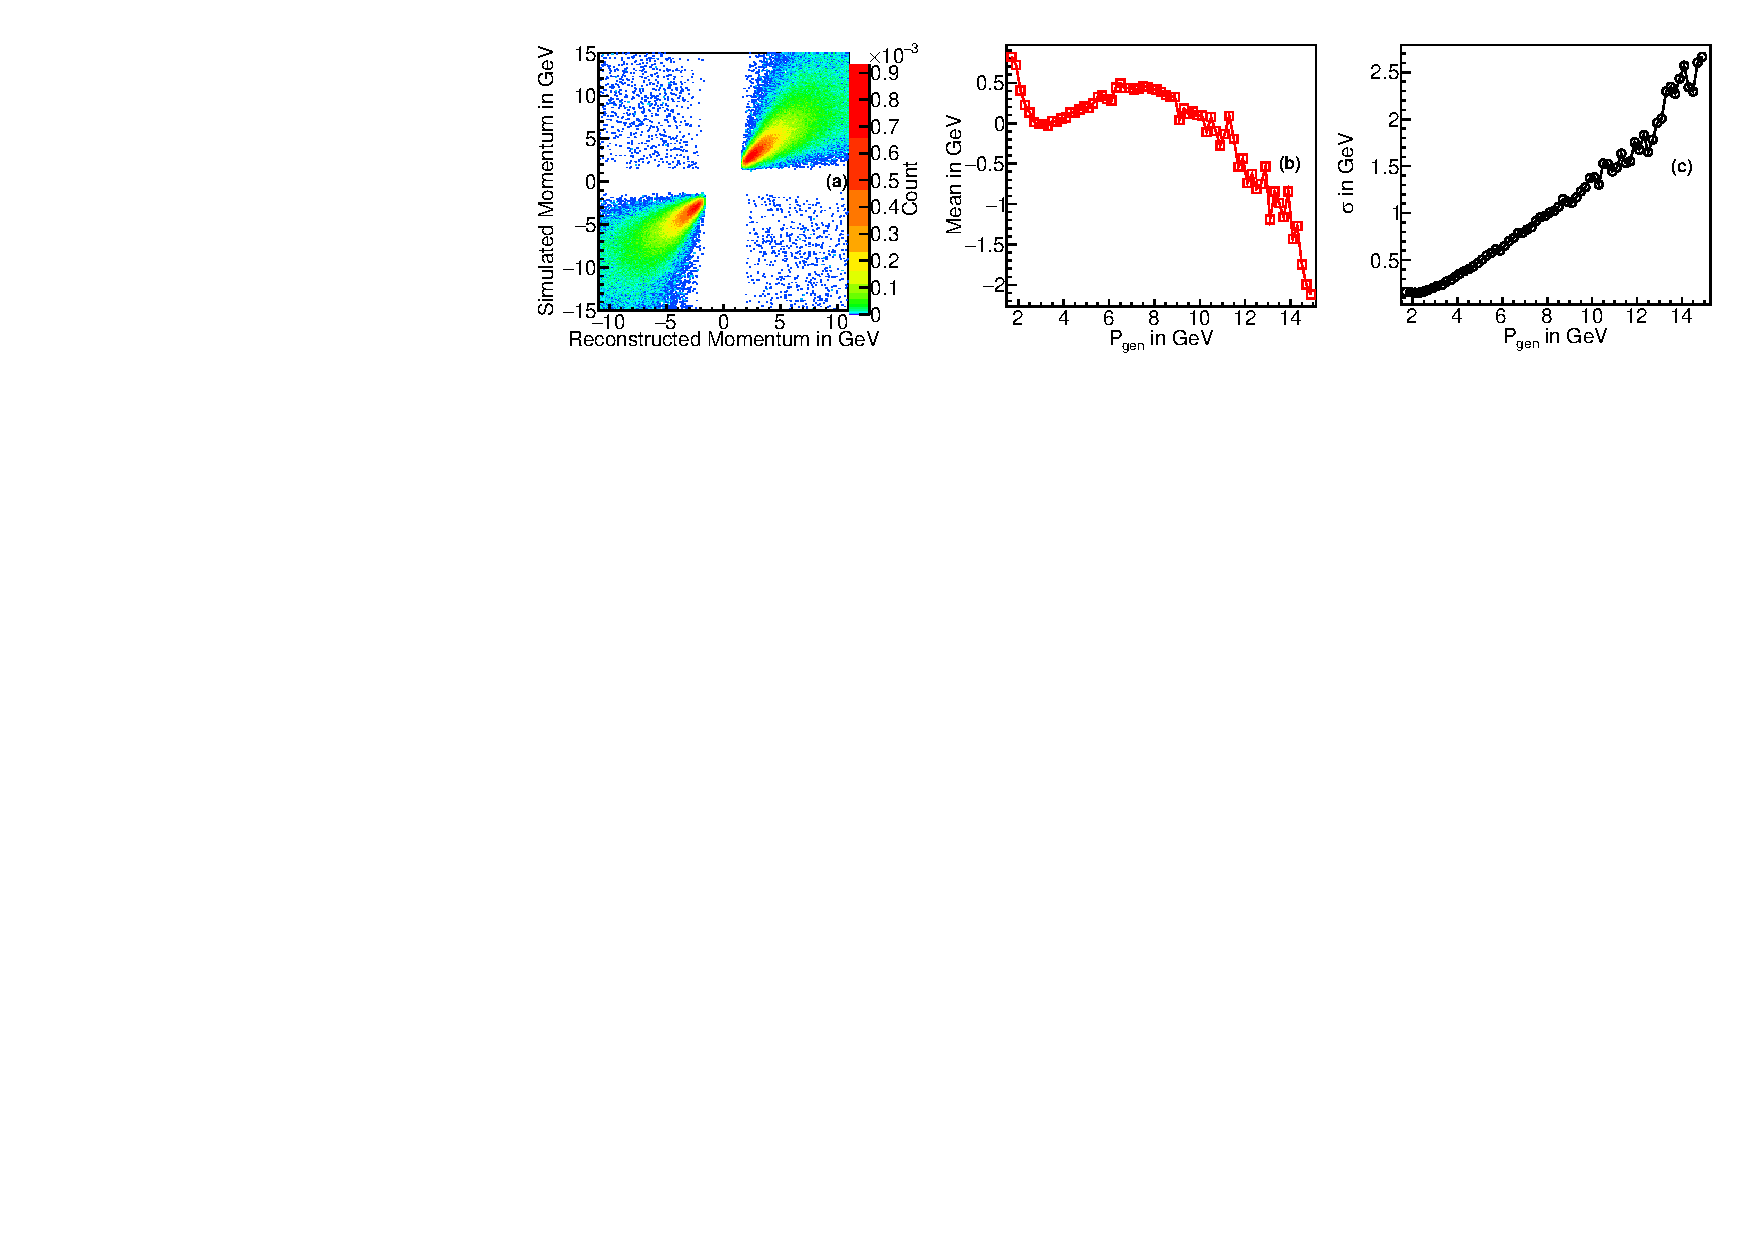
\includegraphics[width=1.\linewidth]{Response_20Layer.pdf}
  \caption{(a) Response Matrix, (b) Mean and (c) $\sigma$ for
    the Engineering Module.}
  \label{fig:eng_mod}
\end{figure}
The efficiency of reconstruction and mis-identification of the charge
of the particles are shown in the Figure~\ref{fig:eng_mod_effi}.
\begin{figure}[h]
  \centering
  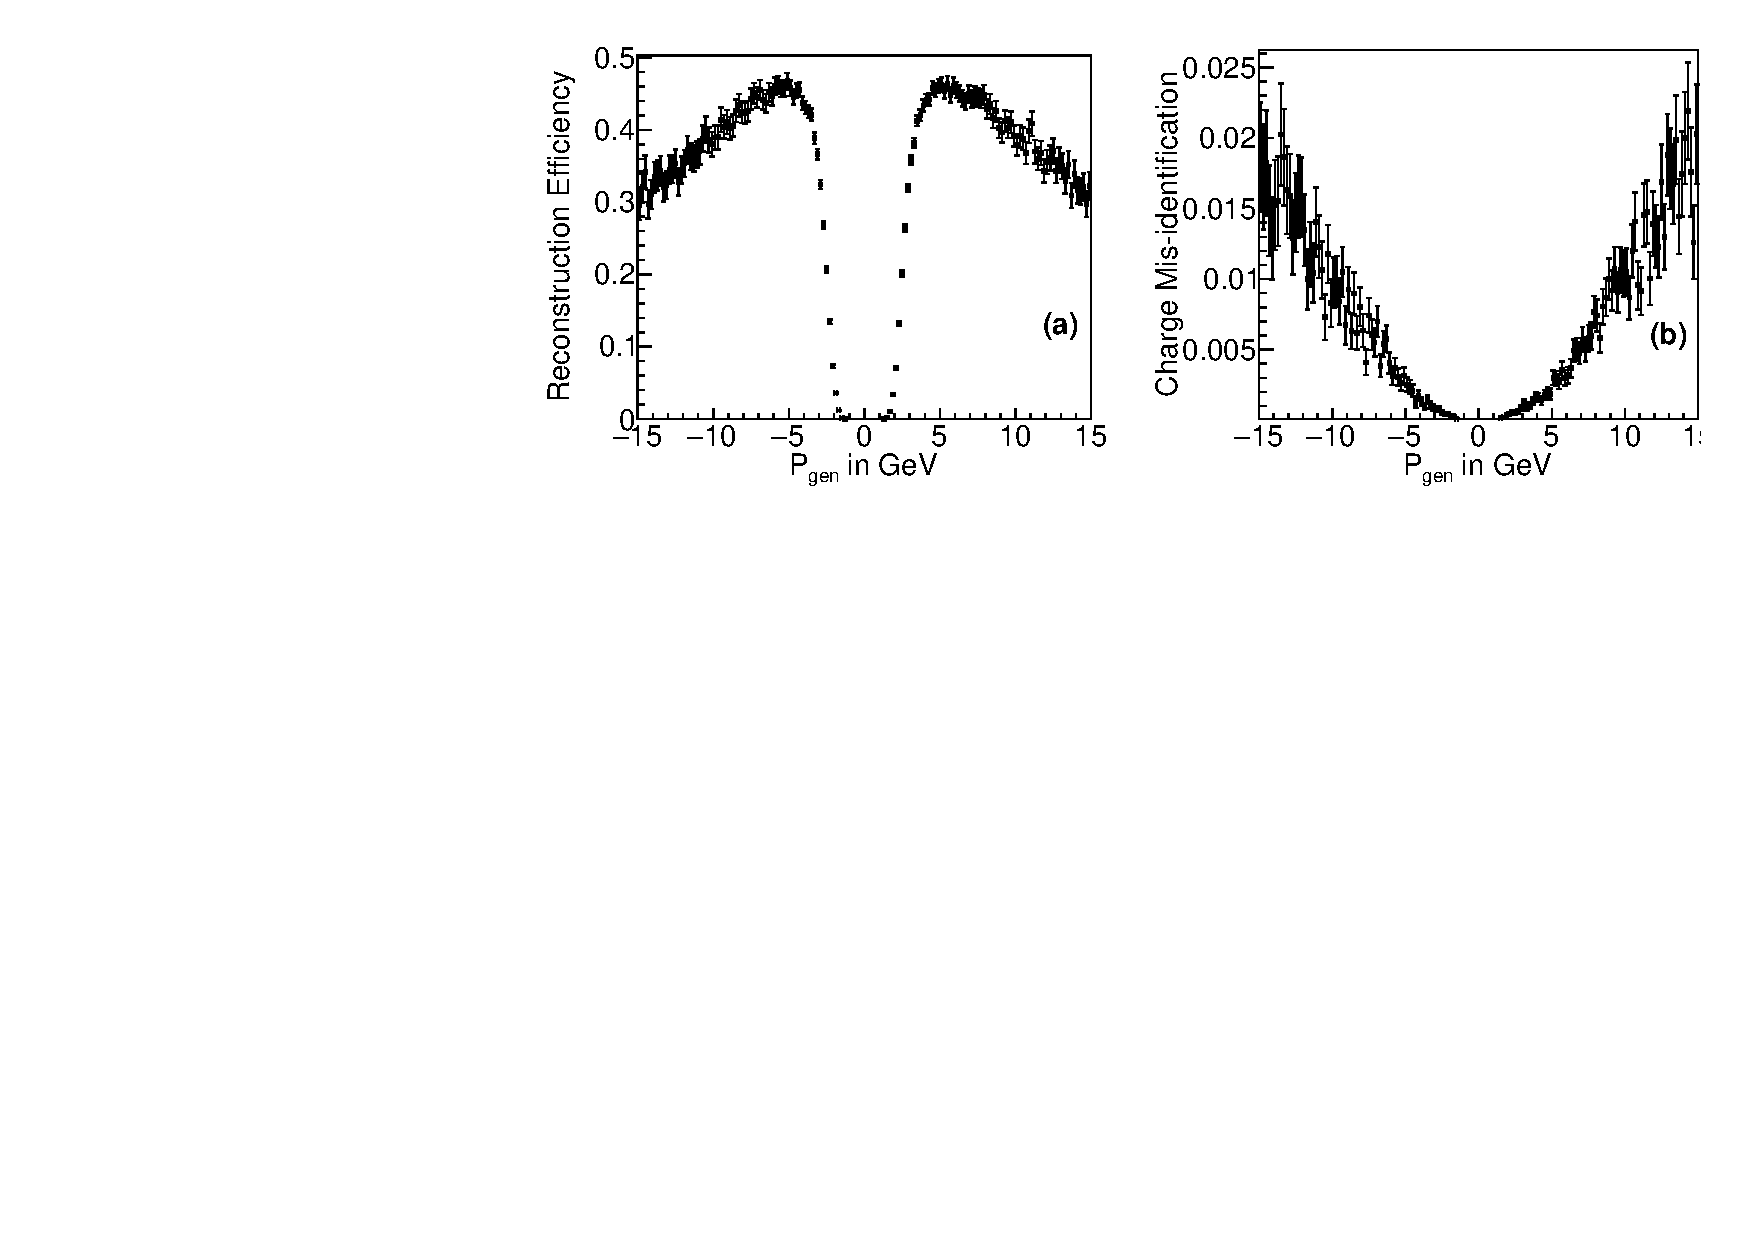
\includegraphics[width=0.8\linewidth]{GMA_effi_misId_20Layer_EM.pdf}
  \caption{(a) Efficiency of reconstruction and (b) Particle charge
    mis-identification plotted against $P_{gen}$ for Engineering Module.}
  \label{fig:eng_mod_effi}
\end{figure}
In the Engineering Module, the momentum should be reconstructed
up-to 12\,GeV along with better charge identification and particle
detection efficiency.

\section{Chapter Summary}
As a part of the ICAL R\&D program, a magnetised detector
(named mini-ICAL) with 10 layers of RPCs interspersed with 56\,mm iron
layers has been built and operational at IICHEP, Madurai situated
near the INO site. The cosmic ray data collected by the detector
setup is used to calculate the charge ratio $(R)$ of the number
of $\mu+$ to $\mu-$ arriving at the Earth's surface.
Using the iterative Bayesian Unfolding technique, the charge ratio
of muons is observed and compared with the BESS-TeV'02 calculation
\cite{bess2002}.
From the study, it is seen that the ratio between $\mu^{+}$ and
$\mu^{-}$ more or less matches in the range of 0.8-3\,GeV.
The reconstruction of momentum beyond this energy range fails due to the
insignificant curvature of the tracks created by the particles, poor
position resolution of RPCs, limited number of tracker layers and
the low-energy cutoff in this detector setup.

A new detector setup with 20 layers of RPC and 8 times larger in volume,
INO Engineering Module is going to be built in few years at IICHEP
Madurai. With more number of detectors, the momentum should be
reconstructed up-to 12\,GeV with the same momentum resolution at
$\sim$3 GeV at present setup. That data will be able to compete
with other experiments in the world to measure the momentum spectra
and charge ratio of cosmic ray muons at the earth's surface.
